\documentclass{article}
\usepackage{graphicx} % Required for inserting images
\usepackage{authblk} % For author affiliations
\usepackage{hyperref} % For hyperlinks
\usepackage[margin=1in]{geometry} % Standard margins
\usepackage{natbib} % For bibliography management
\usepackage{enumitem} % For customising lists
\usepackage{color}
\usepackage{amsmath}
\usepackage{float}
\usepackage{booktabs}
\usepackage{multirow} 
\usepackage{array} 
\usepackage{pdflscape}
 \usepackage{booktabs}
\usepackage{tabularray}
\usepackage{soul}
\usepackage{tabularx}
\usepackage[printonlyused]{acronym}

\newcommand\Fontvi{\fontsize{8}{8}\selectfont}

\newlist{tree}{itemize}{10}
\setlist[tree]{label=-}
\setlistdepth{10} 
\usepackage{comment}

\title{A Workflow for Infectious Disease Modelling}

\author[1]{Sam Abbott}
\author[2]{Xiahui Li$^\dagger$}
\author[3]{Punya Alahakoon$^\dagger$}
\author[4]{Dhorasso Temfack$^\dagger$}
\author[5]{Sabine Van Elsland}
\author[6]{Johannes Bracher}
\author[7]{Felix Günther}
\author[8]{Adrian Lison}
\author[3]{James Hay}
\author[10, 14]{Oliver Eales}
\author[11]{Eben Kenah}
\author[10]{James McCaw}
\author[12]{Mircea T. Sofonea}
\author[7, 13]{Pierre Nouvellet}
\author[14]{Freya Shearer}
\author[1]{Sebastian Funk}
\author[15]{Daniela De Angelis}
\author[16]{Michael J. Plank$^*$}
\author[5]{Anne Cori$^*$}
\author[15]{Anne M. Presanis$^*$}

\affil[1]{London School of Hygiene \& Tropical Medicine}
\affil[2]{School of Mathematics and Statistics, University of St Andrews}
\affil[3]{Pandemic Sciences Institute, Nuffield Department of Medicine, University of Oxford}
\affil[4]{School of Computer Science and Statistics, Trinity College Dublin}
\affil[5]{MRC Centre for Global Infectious Disease Analysis, School of Public Health, Imperial College London}
\affil[6]{Karlsruhe Institute of Technology}
\affil[7]{Robert Koch Institute}
\affil[8]{Computational Evolution, ETH Zurich}
\affil[9]{Nuffield Department of Medicine, University of Oxford}
\affil[10]{School of Mathematics and Statistics, University of Melbourne}
\affil[11]{College of Public Health, Ohio State University}
\affil[12]{University of Montpellier}
\affil[13]{School of Life Sciences, University of Sussex}
\affil[14]{School of Population and Global Health, University of Melbourne}
\affil[15]{MRC Biostatistics Unit, University of Cambridge}
\affil[16]{School of Mathematics and Statistics, University of Canterbury}

\renewcommand{\thefootnote}{\fnsymbol{footnote}}
\footnotetext[1]{$^\dagger$Equal contribution}
\footnotetext[2]{$^*$Equal contribution}

\date{\today}

\begin{document}

\maketitle
\newpage
\begin{abstract}
%Lead: Sam Abbott
Infectious disease models can be used to inform critical public health decisions, yet often don't follow systematic development and validation practices.
The infectious disease modelling community has been slow to adopt rigorous model development and criticism cycles such as the Bayesian workflow, even as these methods become increasingly formalised and widely used in other domains. Recent outbreaks have demonstrated some domain-specific challenges that infectious disease modelling faces, including evolving research questions, emerging data sources, and adapting surveillance systems.
Here, we suggest a workflow for developing and evaluating infectious disease models, building on general Bayesian workflow advice and focusing on domain-specific challenges. This workflow is designed for anyone developing an infectious disease model, and for users of model outputs who need to be able to evaluate modelling studies. At each stage, we provide recommendations based on our experience. We begin by outlining an approach for characterising epidemiological data source properties through a structured checklist. We then present an iterative workflow that extends the Bayesian workflow to the infectious disease domain, with the checklist informing decisions throughout each workflow stage. Our workflow includes defining the research question, development of Directed Acyclic Graph representations of process and observation models in a state-space framework, model modularisation, inference and computation choices, model specification and validation, integration method selection, and real-world considerations. 
Throughout, we identify feedback loops where later decisions impact earlier choices. We also give guidance on using the workflow in evolving settings, such as outbreaks, and on how to report its use. To demonstrate this workflow, we use four schematic case studies that progressively integrate data sources for estimating transmission intensity.
In each one, we give examples of navigating real-world trade-offs between model complexity, computational feasibility, and inferential goals.
These case studies highlight how different data types can provide complementary information but may also impact other workflow choices. 
Our suggested framework emphasises parsimony, modularity, interpretability, and model criticism. By proposing domain-specific workflow practices, we aim to provide a foundation for improving the quality and transparency of infectious disease modelling, particularly during outbreaks where flexible, principled approaches are essential. 
\end{abstract}
\newpage

\tableofcontents
\newpage

\section{Introduction}
% Lead: Sam Abbott

% Paragraph 1: Motivation and Context
Infectious disease models can inform critical public health decisions, yet often don't follow systematic development and validation practices (for recent examples, see \citep{Ward2024-sp, Fyles2024-qz, Abbott2021-delta, Abbott2022-prevalence}).
Responses to the COVID-19 pandemic, the 2022 global mpox clade II outbreak, and the 2014-2016 West Africa Ebola outbreak \citep[e.g.][]{knock2021key, ro2025estimating, Abbott2021-delta, Abbott2022-prevalence, Ward2024-sp, birrell2025real} demonstrated both the value of infectious disease models during outbreaks and the limitations of rapid model development.
These outbreak settings all demonstrate patterns widely found in infectious disease modelling: new data streams emerge over time, surveillance systems evolve to meet changing needs, and models must be developed under time constraints with limited understanding of novel data sources \citep{mccaw2023role}.
The infectious disease modelling community has not widely adopted rigorous model development and criticism practices \citep{box1979robustness}, such as the Bayesian workflow \citep{green2003highly,gelman2020bayesian, nicholson2022interoperability}, which could address these challenges through iterative development, systematic criticism, and principled uncertainty quantification.
This lack of adoption is particularly problematic when integrating multiple data sources, which has been found to improve parameter estimation, reduce uncertainty, and provide more robust evidence for public health decision making, but often requires complex models \citep{deangelis2018analysing, sherratt2021exploring}.

% Paragraph 2: Current Approaches
Current approaches to infectious disease modelling broadly fall into two categories: pipeline methods that fit separate models sequentially for different processes (e.g., separate models for data processing, missing data imputation, and parameter estimation), passing the outputs from one model to the next as an input; and joint modelling approaches that represent these processes in a unified statistical framework \citep{deangelis2018analysing}.
Pipeline approaches offer computational efficiency and modular development, but may propagate errors and fail to capture dependencies and uncertainty \citep{lison2024generative, Ward2024-sp}.
Joint modelling can provide more principled uncertainty quantification and better parameter identifiability, but often requires substantial computational resources and model complexity \citep{russell2024combined, lison2024generative}.
Beyond these choices, there are numerous challenges when integrating multiple data sources, including: detecting and resolving conflicts between data sources, e.g. when different data streams suggest different dynamics; combining data sources with different spatial or temporal resolutions; and navigating branching decision paths where multi-data source integration choices impose model structure constraints \citep{deangelis2018analysing, nicholson2022interoperability}.
Fitting challenges, such as computational intractability, parameter non-identifiability, and the need to approximate ideal model structures for practical inference, further complicate implementation \citep{corbella2022inferring, Ward2024-sp}.
These considerations can impact model design, yet their implications are rarely made explicit in published analyses.
Whilst some work has systematically compared modelling choices for specific case studies \citep{bouman2024bayesian} or provided workflow guidance focused on specific computational frameworks \citep{grinsztajn2021bayesian}, structured guidance remains limited \citep{Behrend2020-au, nicholson2022interoperability, deangelis2018analysing}.

% Paragraph 3: Paper scope and contribution
This paper provides a workflow for infectious disease modelling that applies broadly across model types (e.g. deterministic, stochastic, continuous-time, discrete-time) and model aims, including scenario analysis, disease monitoring, and outbreak response. We give specific guidance for outbreak settings and multiple data source integration, as in our experience, these contexts present particular workflow challenges.
The Bayesian paradigm, combining prior information with data, is a natural framework for infectious disease modelling, since such models usually require at a minimum prior assumptions, more usually both prior information and at least one data stream, and potentially, multiple data streams. Our approach, therefore, builds on established Bayesian workflows \citep{green2003highly,gelman2020bayesian}, which in turn build on Box's scientific method \citep{box1979robustness,Box1980}, extending them for the specific challenges of infectious disease modelling, including evolving research questions, emerging data sources, and time-constrained development.
We advocate for Bayesian thinking throughout the model development process, including model specification, model criticism, and predictive checks, consistent with the model development and criticism cycle required for any statistical model, regardless of inferential framework \citep{box1979robustness}.
We first outline an approach for characterising epidemiological data source properties through a structured checklist, then present an iterative workflow, with the checklist informing decisions throughout each workflow stage.
Our workflow includes defining the research question, developing \ac{DAG} representations of disease and observation processes in a state-space modelling framework, model modularisation, inference and computation choices, model specification and validation, integration method selection, and real-world considerations.
Throughout, we identify feedback loops where later decisions impact earlier choices.
We also provide guidance for using the workflow in evolving settings, such as outbreaks and for reporting modelling using it.
We use four case studies centred on reproduction number estimation to demonstrate this workflow, starting with a single-source baseline, then integrating similar data sources, and finally including data of different types and scales.
By focusing on a common estimation task, we aim to demonstrate broad principles for improving workflow practice that are applicable across a range of infectious disease modelling contexts.
We also provide an example of our suggested data characterisation approach, which we then use throughout our case studies to inform our modelling choices.
Our suggested workflow is designed for anyone who develops infectious disease models, whether in academic research or public health practice, as well as users of model outputs who need to evaluate modelling studies. 
Different readers may wish to engage with the text differently.
We suggest that most readers start by reading the introduction, data sources and characteristics (Section \ref{sec:datareview}), the overview of the workflow (start of Section \ref{sec:workflow}, including the schematics), and the discussion (Section \ref{sec:discuss}).
Depending on the use case, we then suggest either reading through the case studies (Section \ref{sec:casestudies}) and engaging with the full workflow (Sections \ref{sec:research-question} to \ref{sec:reporting}) as needed, engaging with aspects of the workflow most related to current modelling choices, or reading through the full workflow (Section \ref{sec:workflow}) and then working through the case studies (Section \ref{sec:casestudies}) for reinforcement.
% Alternaitve sentence:
% Depending on the use case, readers may then wish to focus primarily on either the full workflow (Sections \ref{sec:workflow}) or the case studies (Section \ref{sec:casestudies}. We provide cross-references between corresponding areas of these sections to assist this.

\section{Data Sources and Characteristics} \label{sec:datareview}
% Lead: Punya Alahakoon

Using multiple data streams has been found to improve parameter estimation and reduce uncertainty in modelling studies for monitoring infectious diseases \citep{deangelis2018analysing, sherratt2021exploring}. While each data source may offer unique advantages, such as timeliness, population coverage, and direct information on some quantities, they also come with distinct limitations, including reporting delays,  measurement noise, or lack of representativeness. There is currently no standardised approach to assess and compare these data sources in terms of their strengths and weaknesses, hindering our ability to compare, integrate, and prioritise data streams effectively. 

The WHO guidelines for integrated surveillance of respiratory pathogens with pandemic potential emphasise the importance of standardised, multi-purpose surveillance systems that also support public health responses and modelling \citep{world2024implementing}. Inspired by these, we propose six overarching characteristics with which to evaluate different data sources in a common framework (Figure \ref{data_characteristics}).  These characteristics are: (1) \textit{metadata}  that encapsulates foundational information about each data stream; (2) the \textit{scope} of a data source, i.e. its representative breadth and epidemiological relevance; (3) \textit{resolution} that describes the granularity and level of detail captured by a data source; (4) \textit{data quality} that encompasses the reliability, accuracy and completeness of the measurements within a data stream; (5) \textit{data utility} that refers to the practical applicability of a data source in informing epidemiological metrics and supporting public-health decision making; and (6)\textit{ practical considerations} that address the feasibility of using a data stream in modelling and surveillance contexts. We define more detailed potential criteria for each of these characteristics as part of the case study and in the Supplementary Materials. 

We propose that these six categories are useful as a guide for the systematic assessment of a data stream's strengths and weaknesses. While the precise structure, relevance, and sub-attributes of each component may vary depending on the specific surveillance and modelling objectives, the key aim of these categories is to promote structured, transparent thinking. We suggest first assessing our checklist for its relevance to a specific research question, then modifying it to better align if necessary. Once happy with the checklist, we recommend reviewing each dataset available in turn, ideally independently, and collating the responses. We then suggest summarising these responses, as demonstrated in our case study, and using them to inform the remainder of the workflow.


\begin{figure}[H] 
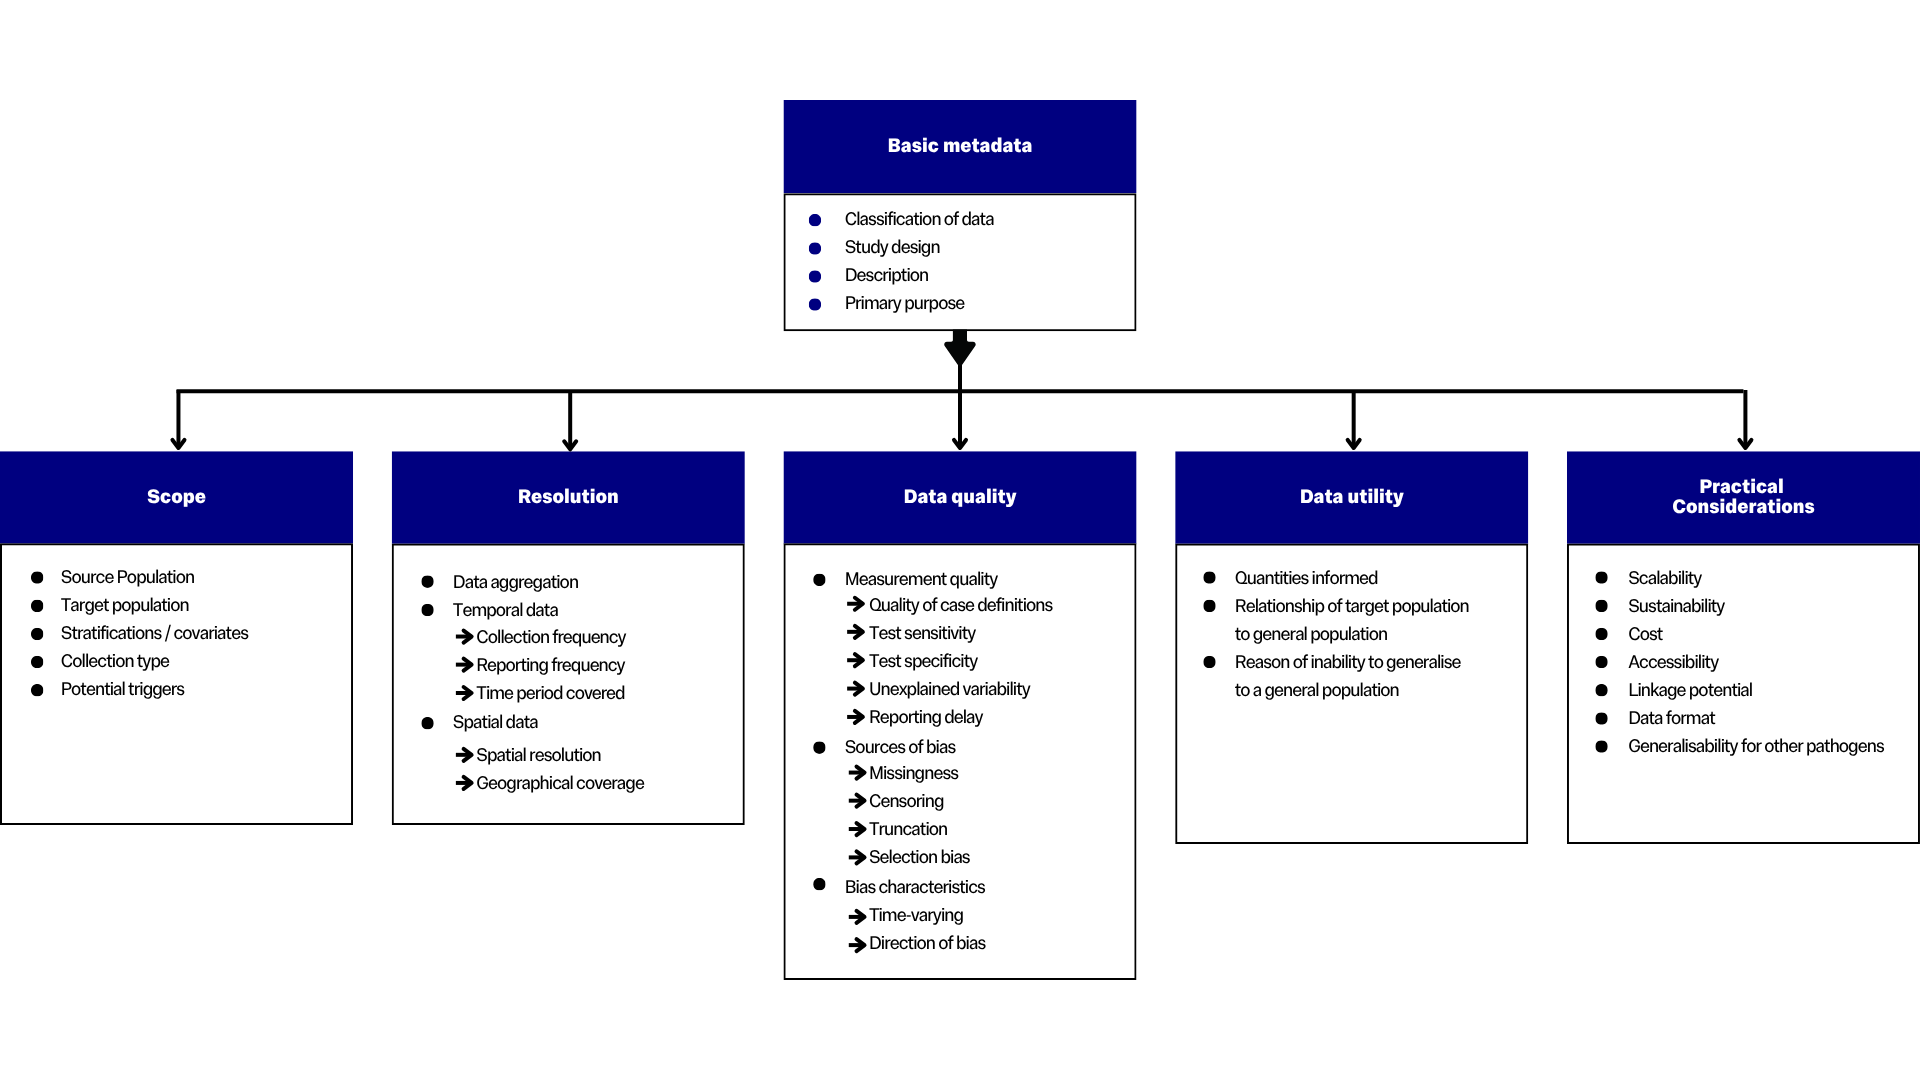
\includegraphics[width=1\linewidth]{figures/Abbott et al figure 1.png}
\centering
\caption{The proposed checklist for characterising a data stream used in infectious disease surveillance and modelling. The six core characteristics---metadata, scope, resolution, data quality, data utility and practical considerations---are illustrated alongside representative attributes that can be used to assess the strengths and limitations of each data source. }
\label{data_characteristics}
\end{figure}


\section{Workflow}
\label{sec:workflow}
% Lead: Sam Abbott

The workflow should be implemented through multiple iterations, starting with high-level considerations and becoming more detailed with each pass, as some steps require decisions in later workflow components. Users may approach this process differently, with some doing fewer, more detailed iterations, and others rapidly working through the workflow initially and then iterating over a greater number of iterations.

We start with clearly defining a \textbf{research question} and \textbf{target estimands} (Section~\ref{sec:research-question}, e.g. time-varying reproduction number, overdispersion parameters). Next, we suggest using a \textbf{\ac{DAG}} to formalise dependencies between variables, thereby defining our model structure. We also suggest using a state space formulation \citep{birrell2018evidence} to modularise the definition of the \textbf{process} and \textbf{observation} models. Starting with the process model (Section~\ref{sec:process}), the corresponding \ac{DAG} represents the underlying latent epidemiological process, i.e. the transmission and related processes, and the processes required to answer the research question. Even if we don't need to explicitly model the transmission or infection process to answer the research question, an initial process \ac{DAG} that includes the transmission process is useful to communicate any simplifying assumptions that are being made.
Our next step is to use the data source characterisation from Section~\ref{sec:datareview} to \textbf{select available data sources} (Section~\ref{sec:data-selection}) that inform our process model. Data sources should be selected based on their expected contributions to the research question. For each data source, we then suggest developing an observation \ac{DAG} for each data source.
The observation model \ac{DAG} (Section~\ref{sec:observation}) links the process model to data, accounting for measurement mechanisms and model misspecification. A key part of our workflow is iteratively refining these representations (Section \ref{sec:refine-dags}), e.g. in light of preliminary results, as an outbreak evolves., or as the research question is updated.
Before continuing with the full model a key step is to develop a \textbf{modularised} version of our joint model (Section~\ref{sec:modularise}) where the model \ac{DAG} is decomposed as much as possible into smaller submodels that can each then be independently verified.

Next, we make \textbf{inference and computation choices} (Section~\ref{sec:fitting}): we select an inference method based on the model structure, and theoretical and practical considerations for each module.
We then decide how to \textbf{implement} our model in the inferential and computational framework chosen (Section~\ref{sec:implementation}), ideally following software development best practices in a probabilistic programming language.
Finally, we apply \textbf{model specification and validation} (Section~\ref{sec:spec-validate}) to each module independently. At this stage, we choose the specific model family to implement our model DAG. Potential model families include deterministic or stochastic differential equations, discrete-time models, and agent-based models.
Our choice is influenced by available expertise, the model structure and our inference and implementation choices. 
In some settings, we recommend using a hybrid approach where, for example, the process model is implemented using differential equations and the observation models are discrete-time statistical models.
Once the model has been specified, we move on to prior specification, parameter identifiability assessment, and prior and posterior predictive checks.

After validating individual modules, we then face key decisions on \textbf{data integration}, namely which modules to combine and how  (Section~\ref{sec:integration}). If combining multiple modules is not beneficial or feasible, we can proceed to the combination of estimates, e.g. where multiple models are used to estimate the effective reproduction number from different data sources, and we combine the different estimates through ensemble approaches. If combining multiple modules is warranted, we select a data integration method and return to inference and computation choices (Section~\ref{sec:fitting}) for the newly combined model.

Throughout this workflow, several feedback loops are possible between steps, so that model development is rarely a single forward pass (see Figure~\ref{fig:workflow}). 
Data characteristics can alter process \ac{DAG} structure: for example, individual-level data requires different representations than population-level data. 
Inference and computation constraints may require approximating or restructuring the process \ac{DAG}.
Practical constraints shape integration choices in multiple ways. 
Teams using incompatible programming languages may need to use non-joint approaches. 
Similarly, computational constraints may favour approximate over exact joint approaches or ensembling independent models.
Alternatively, they can suggest refining the underlying model \ac{DAG}s.
Our choice of model family may also impact our model \ac{DAG}s, as well as the inference approach and implementation method.
Identifiability issues discovered during model validation may require simplifying either the process or observation models. 
The complexity of  integration may also require simplifying models to maintain computational feasibility. 
Finally, conflicts between data sources during integration often reveal model misspecification, requiring revision of earlier assumptions.

Add something about use case counterfactual and forecasting etc.
Add something about model choice.

In the following sections, we discuss each of the workflow steps in more detail and include references to relevant resources for further exploration.

\begin{landscape}
\begin{figure}[htbp]
    \centering
    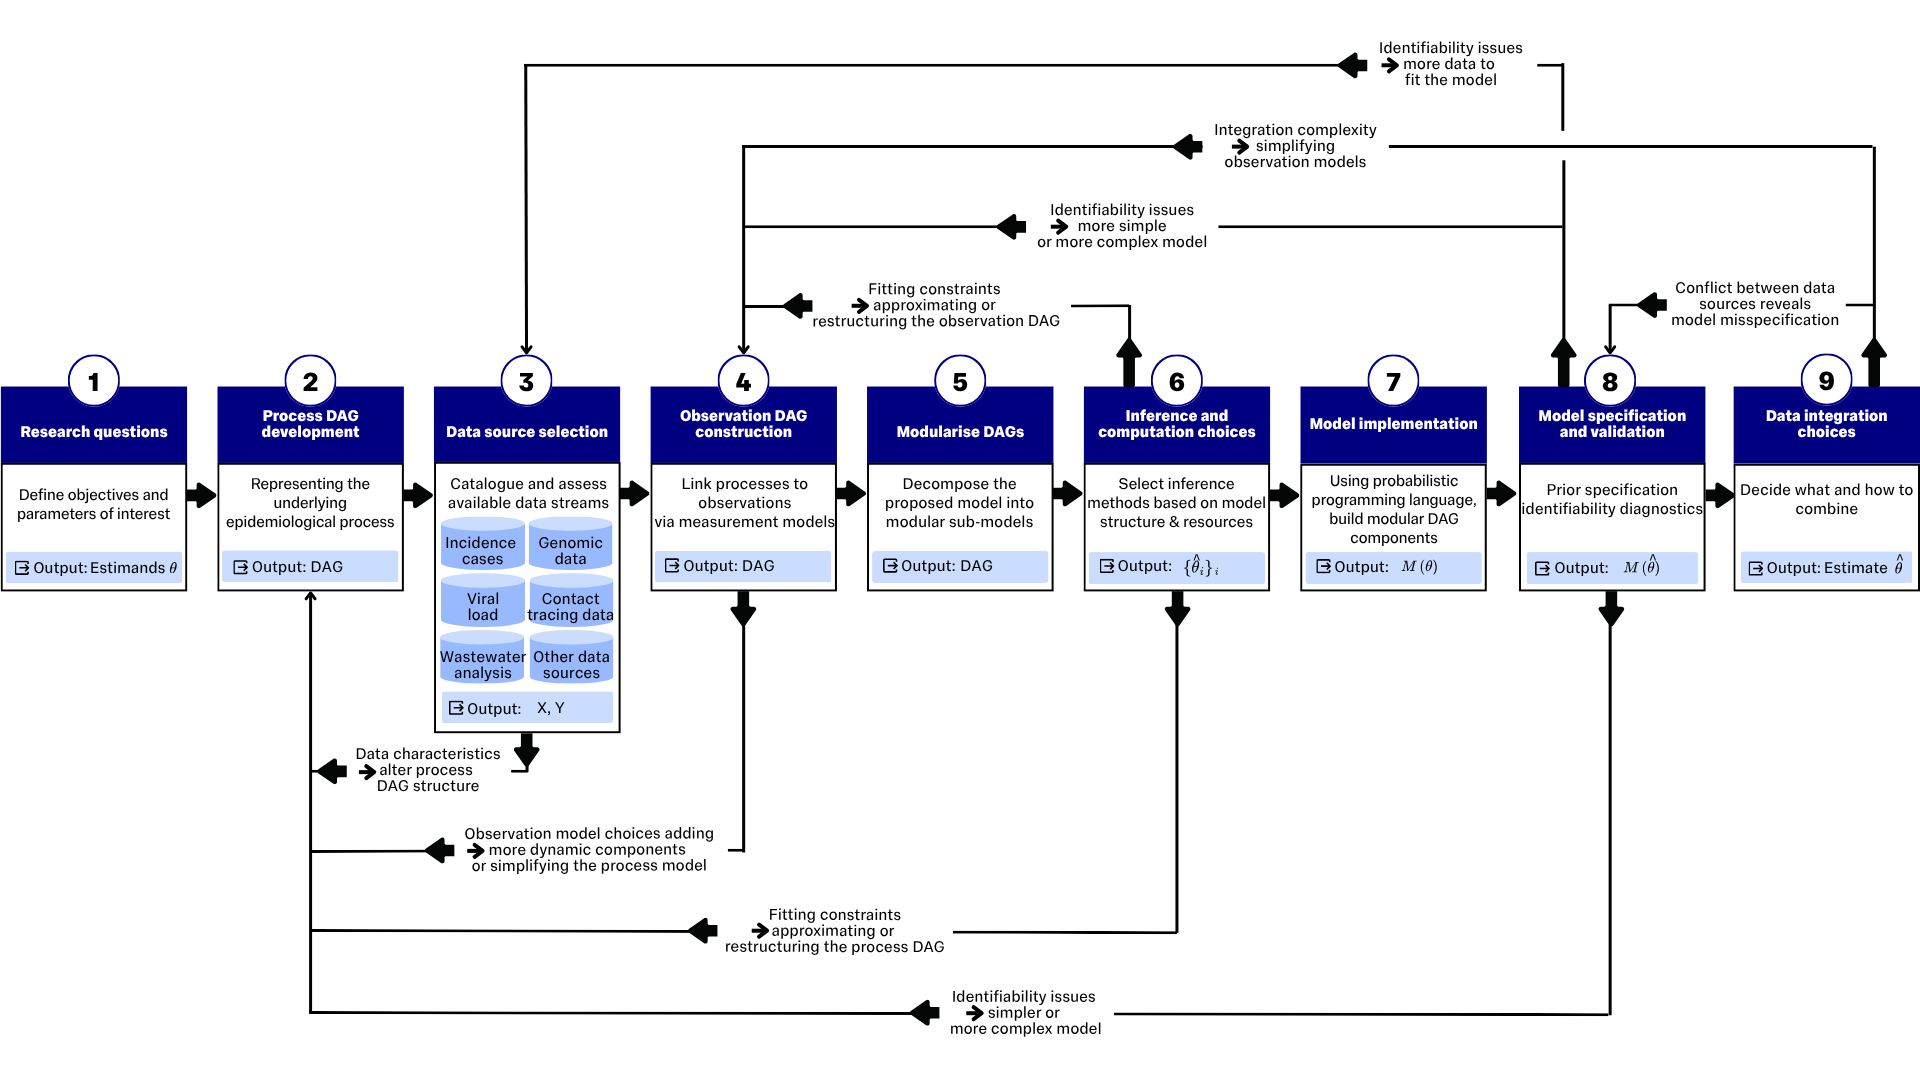
\includegraphics[width = 1.4 \textwidth]{figures/Abbott et al figure 2.png}
    \caption{\textbf{Recommended workflow for integrating multiple data sources in infectious disease modelling.} Key feedback loops from downstream parts of the workflow that impact earlier choices are represented with dashed arrows and boxes.}
    \label{fig:workflow}
\end{figure}
\end{landscape}

\subsection{Research Question and Target Estimands} \label{sec:research-question}

Clearly defining the research question and the epidemiological parameters $\boldsymbol{\theta}$ to be estimated or predicted shapes the entire modelling workflow. Our definitions will result from the main modelling aims, e.g. forecasting hospital admissions or estimating the potential impact of interventions, and are best decided in collaboration with a range of stakeholders \citep{marshall2024when}.
Often, different public health objectives need knowledge of multiple quantities, that require balancing trade-offs. For example, we need both short-term forecasts for operational planning and effective reproduction number ($R_t$) estimates for public communication and interpretability. Our aim is to translate these policy needs into specific target estimands, by understanding how parameters inform decisions \citep{nicholson2022interoperability, who-mosaic-2023}. Policymakers might need to know if transmission is increasing rather than precise values, or whether superspreading drives transmission, to choose between population-wide versus targeted interventions. We recommend defining the scope of an analysis explicitly, including what it cannot address: e.g. a national $R_t$ estimate cannot easily reveal local outbreak dynamics, aggregate case data cannot identify transmission chains, and symptom-based surveillance may not detect mild infections.
These limitations help shape stakeholder expectations and prevent misuse of results.

Note that our research questions are likely to evolve throughout outbreaks. Early outbreak questions often focus on growth rates and severity using limited case data. As surveillance expands, questions might shift, for example, to understand variant dynamics, requiring genomic data integration; then to quantifying population immunity, needing serological data \citep{bhatia2023lessons,shearer2024opportunities}. See Section \ref{sec:outbreak} for more on dealing with evolving outbreak settings.

Add something about use case i.e. counterfactual and forecasting

\subsection{Process DAG Development} \label{sec:process}

Epidemic processes can often be described using Markovian state-space models \citep{birrell2018evidence}, where latent states $\boldsymbol{X}_t$, e.g. the number of infectious individuals $I_t$, evolve over (discrete) time according to dynamics 
\begin{align*}
\boldsymbol{X}_{0} \mid \boldsymbol{\theta} & \sim p(\boldsymbol{x}_0 \mid \boldsymbol{\theta}) \\
\boldsymbol{X}_{t} \mid \boldsymbol{X}_{t-1}, \boldsymbol{\theta} & \sim p(\boldsymbol{x}_t \mid \boldsymbol{x}_{t-1}, \boldsymbol{\theta})
\end{align*}
governed by (a subset of) parameters $\boldsymbol{\theta} \in \boldsymbol{\Theta}$, e.g. the force of infection $\lambda_t$. The state-space representation is completed by the observation process (Section~\ref{sec:observation}), where data are observed conditional on the current state of the system, governed by observation model parameters (a subset of $\boldsymbol{\theta}$, e.g. a reporting rate):
$$
\boldsymbol{Y}_{t} \mid \boldsymbol{X_t}, \boldsymbol{\theta} \sim p(\boldsymbol{y}_t \mid \boldsymbol{x}_t, \boldsymbol{\theta}) 
$$
so that the full joint probability model in a Bayesian framework of the random variables $(\boldsymbol{\Theta}, \boldsymbol{X_{0:T}}
, \boldsymbol{Y_{1:T}})$ is
$$
p(\boldsymbol{x}_{0:T}, \boldsymbol{y}_{1:T} , \boldsymbol{\theta}) = p(\boldsymbol{\theta})p(\boldsymbol{x}_0 \mid \boldsymbol{\theta})\prod_{t=1}^T p(\boldsymbol{x}_t \mid \boldsymbol{x}_{t-1}, \boldsymbol{\theta})p(\boldsymbol{y}_t \mid \boldsymbol{x}_t, \boldsymbol{\theta}).
$$
The state-space framework links the process model to observed data. Although in general state-space models represent stochastic processes over time, models that include deterministic relationships or that are static can be seen as special cases \citep{birrell2018evidence}. 

State-space models can be visualised using \ac{DAG}s, which represent the joint distribution of all variables (both observed $\boldsymbol{Y}_t$ and latent $\{\boldsymbol{X}_t, \boldsymbol{\theta}\}$) in a model, visualised as nodes. This joint distribution is factorised into the distribution of each variable conditional on its parent nodes, with directed edges representing these dependences. This formal representation makes conditional independence assumptions explicit and easily readable from the \ac{DAG}, with the basic assumption being that any node is conditionally independent of its non-descendants given its parents \citep{lauritzen1996graphical}. We recommend using \ac{DAG}s in a state-space framework for structuring infectious disease models because they separate the components which are key to our research question and that influence transmission from how we observe them. 
For example, in wastewater modelling, the shedding process is usually part of the observation \ac{DAG}; however, if we think that viral material shed into the environment could also cause infections, it would become part of the process model.
This separation enables modular model development where process components can be reused across different surveillance contexts \citep{nicholson2022interoperability}.
Some common elements of process \ac{DAG}s might be population structure, contact patterns, infection progression, and immunity dynamics \citep{deangelis2018analysing}. 
Our aim when constructing a process \ac{DAG} is to translate our research question and target estimands into structures that can be evaluated, communicated, and refined.
Rather than starting from scratch, we recommend aiming to adapt established epidemiological models for similar pathogens or transmission routes, modifying components as outbreak-specific data emerges \citep{gelman2020bayesian}.
We can either begin model development simply and add complexity, or start with a comprehensive model and simplify to essential components \citep{gelman2020bayesian}.
Generally, we recommend starting with a simple representation of core transmission dynamics, then iteratively refining as understanding improves or as needed by other parts of the workflow.
For example, early outbreak \ac{DAG}s might represent homogeneous mixing, while later versions could incorporate age structure, spatial heterogeneity, or variant dynamics.
However, this workflow is not always possible (e.g. when starting with an already developed model), and so a more complex initial process model may need to be specified, which can then be simplified in later steps, e.g. if the data don't allow identification of all parameters.
Biological mechanisms often shape the process \ac{DAG} structure. For example, incubation periods create latent states between the susceptible and infectious states, with the numbers in each state represented by a node in the \ac{DAG}; generation time distributions determine numbers of newly infected individuals with this dependence represented by a directed edge; and waning immunity adds nodes representing transition rates from recovered back to susceptible compartments.
These structural choices directly affect transmission dynamics and parameter identifiability (Section~\ref{sec:spec-validate}).

\subsection{Data Source Selection} \label{sec:data-selection}

With the process \ac{DAG} and target estimands defined, we next select appropriate data sources, drawing from the data review (Section~\ref{sec:datareview}), based on their characteristics and the specific epidemiological quantities they inform.
For example, case data can be a proxy for infection incidence with reporting delays and ascertainment bias, hospitalisations capture severe outcomes, and wastewater indicates population-level pathogen shedding, independent of healthcare-seeking behaviour.
In principle, integrating multiple data sources should enhance the identifiability and precision of parameter estimates \citep{deangelis2018analysing, lison2024generative, russell2024combined, birrell2025real}. In practice, however, data integration may pose challenges. 
These include inconsistencies due to unaccounted biases \citep{presanis2013conflict,knock2021key, Ward2024-sp, corbella2022inferring}; computational complexity \citep{corbella2022inferring}; and operational constraints during an outbreak emergency \citep{mccaw2023role}.
We therefore recommend starting with minimum data requirements for target estimands and then expanding systematically. 
We also suggest picking initial data sources that are expected, based on their characteristics, to be the most straightforward to model.
We then recommend evaluating complementarity among selected data sources, by assessing whether they provide independent signals on different parameters. For example, wastewater surveillance may provide early warning of outbreaks, while clinical surveillance provides individual-level severity data. Multiple data sources may alternatively inform the same parameter, reinforcing evidence on that parameter and introducing some redundancy. While this redundancy can enhance precision, consistent with meta-analytic principles \citep{deangelis2018analysing,borenstein2021introduction}, it can also increase model complexity.

Finally, we recommend prioritising data sources based on their expected information gain relative to implementation cost and feasibility. ``Value of information'' methods \citep{jackson2019value,heath2024value} can formally guide whether additional data would meaningfully improve precision. However, for complex models especially, identifiability may only become evident after fitting an initial version.

\subsection{Observation DAG Construction} \label{sec:observation}

We now construct the observation process component of the state-space model, again using \ac{DAG}s to map how latent epidemiological processes generate the observed data $\boldsymbol{Y}_t \mid \boldsymbol{X}_t, \boldsymbol{\theta}$, with complexity shaped by the target estimands and selected data sources \citep{deangelis2018analysing,birrell2018evidence}.
We propose building these \ac{DAG}s by thinking through each intermediate step that leads from the process model to observation and then proposing the simplest model that can plausibly represent these observation processes.
In future feedback loops, this representation can then be refined as needed to capture the observed data better.
For example, for clinical surveillance data, steps may include symptom-based healthcare seeking, obtaining a sample to be tested, testing in a laboratory, and reporting; whilst for wastewater surveillance they may describe pathogen shedding, sewage transport, lab processing, and quantification.
Where a step is expected to introduce delays, biases, or induce missing data that affect inference, our observation model should explicitly account for them. For example, we need to adjust for reporting and other delays that create temporal misalignment between transmission events, disease sequelae and observations  \citep{seaman2022nowcasting}. It is also important to distinguish between different missing data mechanisms since random missingness and systematic under-ascertainment require different handling \citep{sherratt2021exploring}. Often, we may  also need to account for time-varying observation probabilities, e.g. driven by changes in testing capacity, healthcare seeking or surveillance intensity. Observation components should ideally be modular and replaceable  \citep{gelman2020bayesian}. For example, initial Poisson noise models may need to become negative binomial to account for overdispersion in reported counts. This flexibility of approach reduces initial specification burden whilst enabling systematic refinement.
As for the process \ac{DAG}, we recommend starting with a simplified observation DAG and iteratively increasing complexity as required by the research question and later stages of the workflow.

Whilst it is hard to give general guidance as to the appropriate observation model for a given setting it is useful to consider some examples.
Estimating population-level transmission requires simpler observation models than understanding variant-specific dynamics or age-stratified patterns.
Individual-level data enables different, more realistic, observation models compared to aggregated reports.
An important challenge when constructing the observation model using multiple data sources is how we handle dependencies between them. For example, data streams may relate to the same underlying epidemiological process; or surveillance systems may have dependencies i.e., individuals may be captured by two or more systems. Developing a \ac{DAG} will help us identify such dependencies.
Finally, we must account for hierarchical structure and population heterogeneity when demographic subgroups are present in the data or are central to the research question. We can validate our understanding of observation processes when we have multiple observation \ac{DAG}s for the same underlying process by checking whether different data streams imply consistent transmission dynamics when properly integrated.

\subsection{Refining the model DAGs} \label{sec:refine-dags}

After mapping data sources and constructing our observations \ac{DAG}s, we revisit our process and observation \ac{DAG}s to ensure alignment between what we want to model and what our data can support.
This step of the workflow aims to create a single joint \ac{DAG} of our state-space model composed of our process and observation \ac{DAG}s.
Data availability can drive both increases and decreases in process model complexity.
For example, contact tracing data with identified transmission pairs allows us to shift from population-level compartmental models to individual-based representations that capture heterogeneous mixing patterns.
Conversely, discovering that surveillance only provides aggregate counts may require collapsing a planned age-structured model into a simpler model.
Strong prior information can sometimes be used to compensate for data limitations, providing a further source of evidence, and so supporting otherwise difficult to identify model specifications.
For example, well-informed priors about transmission parameters from previous outbreaks might support maintaining a risk stratified transmission model even when we have limited data; and detailed knowledge about age-specific contact patterns from previous studies could support using age structure, even if we only have total case counts.
Note that assuming fixed parameter values, common in mechanistic modelling literature, is effectively placing infinitely strong priors: we advocate avoiding such fixed values where possible in favour of appropriately uncertain prior distributions.
Temporal resolution affects what variation can be identified rather than what can be modelled: we can always build a daily-scale model, but weekly surveillance data will usually inform weekly or longer-term patterns, not daily fluctuations.
Additional \ac{DAG} iteration typically occurs at key workflow stages (Figure~\ref{fig:workflow}), such as during model specification when identifiability issues emerge, during validation and/or data integration, when misalignment between model structure and data patterns is exposed, or due to practical or theoretical considerations related to model fitting \citep{corbella2022inferring}.
Each iteration should address specific problems rather than making arbitrary changes.

In some cases, we may be unable to use domain knowledge or reasoning to produce a single valid DAG and instead have several candidates for either or both the process and observation \ac{DAG}s. For example, independent teams working on a similar problem might generate different \ac{DAG}s, particularly when mechanisms are not well-known or the data-generating process is poorly reported. If so, we proceed through the remainder of the workflow with each candidate \ac{DAG}, comparing them in \ref{sec:spec-validate} and potentially integrating them in \ref{sec:integration}.

\subsection{Modularising DAGs} \label{sec:modularise}

After selecting data sources and developing and iterating on our \ac{DAG}s, we decompose our proposed model into modular sub-models (we may already have these modules from generating our observation process \ac{DAG}s).
Each sub-model should be as simple as possible, ideally including the process DAG and a single observation DAG, therefore depending on a single data source.
We may need to make additional simplifying assumptions, which will be relaxed during the data integration step.
For particularly complex models, we recommend starting with an even more modular approach, with the process and observation DAGs being initially treated separately from each other or even modularising them still further into lower-level components (likely needing to use simulated data and inputs for this step and, as with other modularisation steps, making simplifying assumptions).

We start with simple sub-models as it is easier to diagnose issues such as poor fit, model misspecification or convergence issues for modules than for complex models.
We then add complexity incrementally, only as far as needed.
This modularisation facilitates detection of inconsistencies or conflicts between data sources \citep{presanis2013conflict,manderson2023combining} and offers computational advantages over joint modelling \citep{deangelis2018analysing,goudie2019joining,gelman2020bayesian,nicholson2022interoperability}.

We apply the following workflow stages (Inference and Computation Choices, Implementation Considerations, Model Specification and Validation) to each module independently, then, if validated, we proceed to Data Integration Choices (Section \ref{sec:integration}) to determine how to combine them.
The integrated model may then require additional cycles through the workflow.

\subsection{Inference and Computation Choices}\label{sec:fitting}
% Lead: Xiahui and Dhorasso with support from Sam Abbott

Inference for infectious disease models involves estimating parameters $\boldsymbol{\theta}$ from observed data $\boldsymbol{y_{1:T}}$.
We assume these data arise from a probabilistic model with a likelihood function $p(\boldsymbol{y_{1:T}} |
  \boldsymbol{\theta})$ that links parameters to data as specified in our process and observation \ac{DAG}s (Sections \ref{sec:process} and \ref{sec:observation}).
Bayesian inference, our recommended approach, updates prior beliefs $p(\boldsymbol{\theta})$ with the likelihood to obtain posterior distributions $p(\boldsymbol{\theta} | \boldsymbol{y_{1:T}}) \propto p(\boldsymbol{y_{1:T}}|\boldsymbol{\theta}) p(\boldsymbol{\theta})$, providing principled uncertainty quantification.
We have found that inference requires balancing model complexity, computational feasibility, likelihood tractability, and available expertise.
For this reason, we structure inference and computation decisions through four stages: model complexity, selecting inference methods, implementation, and diagnostics (Figure \ref{fig:fitting}). 
These choices create feedback loops within the workflow where computational constraints may require approximating or restructuring earlier \ac{DAG} specifications.
This section provides an overview of these considerations.

\begin{figure}[htbp]
    \centering
    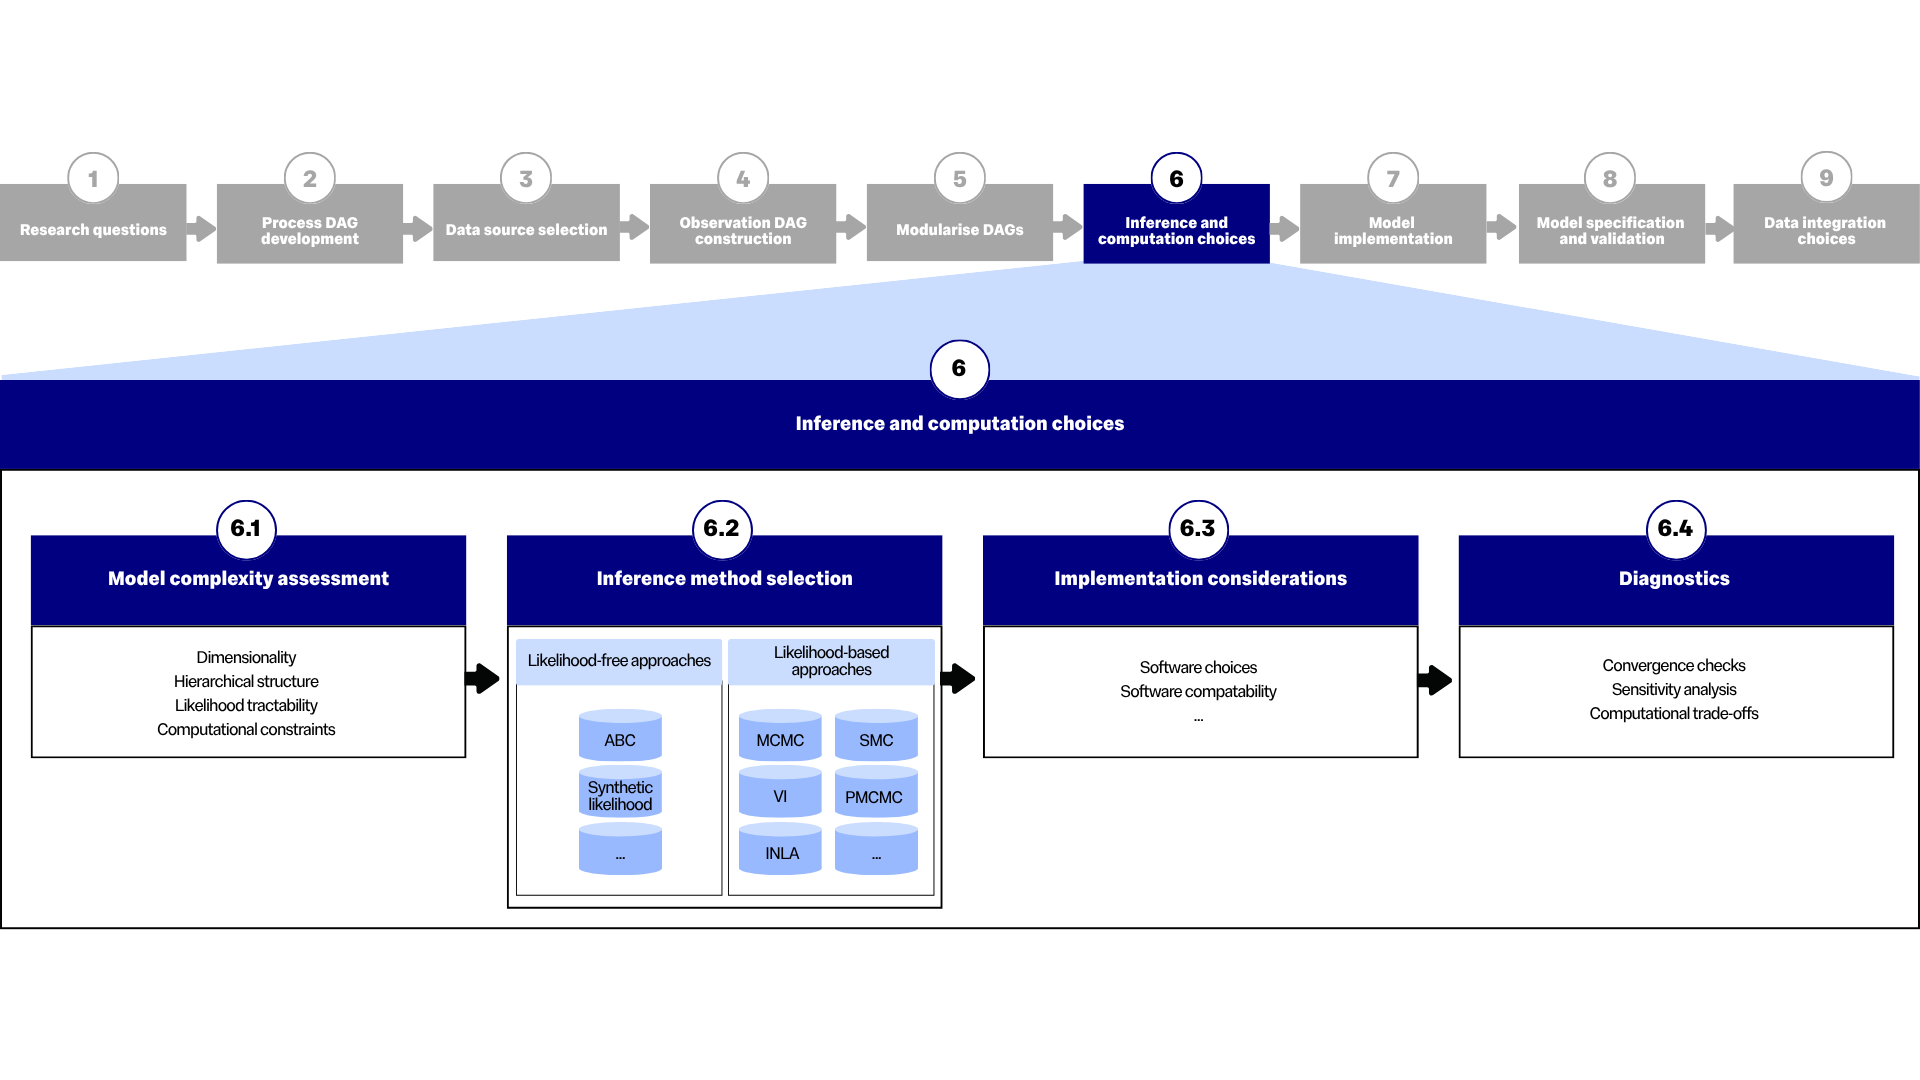
\includegraphics[width=\textwidth]{figures/Abbott et al figure 3.png}
    \caption{\textbf{Inference and computation choices workflow for integrating multiple data sources in infectious disease modelling.} The workflow contains four components: Model Complexity Assessment (6.1) evaluates dimensionality, hierarchical structure, likelihood tractability, and computational constraints; Inference Method Selection (6.2) chooses between likelihood-free approaches and likelihood-based methods; Implementation Considerations (6.3) address software choices and compatibility requirements; and Diagnostics (6.4) involve convergence checks, sensitivity analysis, and computational trade-offs. For simplicity, feedback loops are omitted in this schematic. For a complete representation of feedback mechanisms, see Figure \ref{fig:workflow}.}
    \label{fig:fitting}
\end{figure}

\subsubsection{Model Complexity Assessment}

Before determining the inference approach, it is important we assess the complexity of the model.
Parameter dimensionality and structure are key to method selection as low-dimensional problems with fewer than 10 parameters require different approaches than problems with hundreds or thousands of parameters (see ``Handles high-dim. params.?'' in Table \ref{tab:methods_comparison}).
Similarly, strongly correlated parameters, discrete parameter spaces, or mixed continuous-discrete problems each impact which methods we can use or how they are implemented.
We also need to consider the number of latent variables, such as unobserved infection times, individual-level disease states, or spatially varying transmission rates.
When there are many latent variables relative to observed data, computational feasibility becomes a constraint that rules out certain approaches.
The tractability of the likelihood also determines which methods can be applied.
Key questions we typically ask ourselves include whether we can write the likelihood $p(\boldsymbol{y_{1:T}}|\boldsymbol{\theta})$ analytically, evaluate it numerically at reasonable cost, or differentiate it with respect to parameters.
As an example, models with stochastic differential equations or discrete event processes often lack tractable likelihoods, ruling out methods that require likelihood evaluation or gradients.

\subsubsection{Inference Method Selection}

Numerous methods and algorithmic variants exist within each broad class of inference approach, with distinct computational characteristics and practical trade-offs.
Rather than adopting a universal approach, our choice should be tailored to the specific modelling context, inferential goals, and the expertise of our team.
The following gives guidance to selecting a method, but does not cover all settings.

Gradient-based \ac{MCMC} approaches represent our preferred methods when applicable due to their combination of efficiency, reliability, and ease of use \citep{gilks1995markov, lekone2006statistical}.
\ac{MCMC} methods generate samples from the posterior distribution by constructing a Markov chain that converges to the target distribution, providing a flexible framework for Bayesian inference when analytical solutions are unavailable.
\ac{HMC} leverages gradient information for efficient \ac{MCMC} exploration of differentiable likelihoods, with its adaptive variant \ac{NUTS} representing our default recommendation for models with continuous parameters, or where discrete parameters can be marginalised out \citep{duane1987hybrid, hoffman2014no, andrade2020evaluation}.
When implementing gradient-based methods, the automatic differentiation method can have a substantial impact: forward-mode differentiation suits models with few parameters (typically fewer than 10), whilst reverse-mode differentiation scales better for high-dimensional parameter spaces \citep{baydin2018automatic, andelfinger2023towards}.
In our experience, when it is possible to  do so testing different automatic differentiation options can greatly speed up model development.
When full uncertainty quantification is less critical, \ac{VI} approximates the posterior by optimising tractable surrogate distributions, offering fast approximation with modern variants like Pathfinder \citep{blei2017variational, chatzilena2019contemporary}.
These approaches can often be useful for prototyping, but we have found that they need to be used with care as they can mask issues with models that less approximate approaches identify.

Sampling-based approaches become necessary when gradients are unavailable.
Standard sampling-based \ac{MCMC} methods including Metropolis-Hastings and Gibbs sampling handle discrete or mixed parameter spaces \citep{hastings1970monte, geman1984stochastic, gilks1995markov}.
For discrete parameters, we recommend considering whether marginalisation is possible before resorting to sampling, as analytical integration can significantly improve efficiency and mixing.
Parallel tempering extends these methods to multimodal posteriors by running multiple chains at different temperatures, with modern implementations available in packages like Pigeons.jl \citep{surjanovic2023pigeons}.
For models in which the latent state dimension grows over time, as in state-space models, \ac{MCMC} becomes increasingly inefficient.

\ac{SMC} methods, or particle filters, offer a natural alternative in models with latent states. These methods approximate distributions, e.g. the posterior distribution of latent states, over time using many parallel simulations (referred to as particles), each weighted according to how well it matches the observed data. A key property of \ac{SMC} is that it provides an unbiased estimate of the likelihood, which makes it particularly useful when embedded in parameter inference schemes \citep{doucet2001introduction}. \ac{PMCMC} exploits this by combining \ac{SMC} with \ac{MCMC} for joint state–parameter inference \citep{andrieu2010particle, endo2019introduction}, while \ac{SMC$^2$} extends the idea to fully sequential Bayesian updating as observations accumulate \citep{chopin2013smc2, TEMFACK2025100847}. A significant advantage of  \ac{SMC} methods is that they enable online Bayesian updating as new data arrive, making them well-suited for real-time epidemic tracking \citep{birrell2020efficient, storvik2023sequential}. 
\ac{PMCMC} is widely used for infectious disease modelling including in the \ac{POMP} and ODIN ecosystems \citep{king2016statistical, fitzjohn2021reproducible}. Despite these strengths and being widely used, particle-based methods face challenges such as particle degeneracy (where few particles carry most weight) and memory demands with long time series. Table \ref{tab:methods_comparison} summarizes their main advantages and limitations.
Approximate Bayesian inference methods provide efficient alternatives for specific model structures.
\ac{INLA} offers a computationally efficient method for approximating posterior marginals in latent Gaussian models, making it particularly effective for spatio-temporal disease models with spatial correlation structures \citep{rue2017bayesian}.
This method excels when models can be reformulated with latent Gaussian components but struggles with non-Gaussian latent structures.

Beyond Bayesian approaches, \ac{MLE} provides both point estimates for model parameters and uncertainty quantification in the form of standard errors and confidence intervals. The \ac{MLE} converges to the true parameter as the sample size increases and is asymptotically efficient, achieving the lowest possible variance among unbiased estimators \citep{myung2003tutorial, baltazar2024maximum}. However, uncertainty quantification for complex models can be challenging in a frequentist framework without resorting to computationally expensive bootstrapping.
Profile likelihood methods extend \ac{MLE} by examining the likelihood surface for individual parameters whilst optimising over others, providing confidence intervals without full posterior sampling \citep{tonsing2018profile, plank2024structured}.
All of these approaches struggle to incorporate domain knowledge to the extent that priors allow for Bayesian methods, and so we in general, don't recommend them outside of prototyping and where other approaches are not available.

We think that traditional likelihood-free approaches are methods of last resort due to their computational demands and limited diagnostic capabilities.
These simulation-based methods bypass likelihood evaluation entirely, instead using model simulations to approximate the posterior distribution.
\ac{ABC} approximates the posterior distribution by accepting parameter values that generate simulated data close to the observed data under a predefined distance metric, whilst \ac{SL} methods approximate the likelihood by assuming Gaussian distributions for summary statistics \citep{beaumont2002approximate, wood2010statistical, price2018bayesian}. 

Recent advances in machine learning-augmented inference show promise, with neural network-based summary statistic construction \citep{raynal2019abc} and deep learning phylodynamic methods \citep{voznica2022deep} providing potential alternatives to traditional likelihood evaluation. Alongside these advances, recent developments such as generalized adaptive \ac{HMC} \citep{bou2025within}, gradient-free \ac{MCMC} algorithms \citep{bou2025no}, microcanonical \ac{HMC} \citep{robnik2023microcanonical}, and normalizing flows \citep{papamakarios2021normalizing} are making high-performance tools increasingly accessible for applied researchers. As these next generation techniques continue to develop, it is important to revisit and refine current methodological recommendations to ensure they remain aligned with emerging computational capabilities.

\begin{landscape}
\begin{table}[ht]
\renewcommand{\arraystretch}{1.2}
\centering
\caption{\textbf{Comparison of Likelihood-Based and Likelihood-Free Fitting Methods.} 
This table focuses on foundational algorithms. More recent methodological advancements that build upon these classical approaches are discussed in Section~\ref{sec:fitting}. ``PPL'' stands for Probabilistic Programming Languages. For this review, PPL examples include Stan, PyMC, JAGS, NIMBLE, Turing.jl, etc.``PPC'' stands for posterior predictive checks.}
\label{tab:methods_comparison}
\small
\begin{tabular}{@{}p{3.5cm}p{1.5cm}p{1.5cm}p{2.2cm}p{2.2cm}p{1.5cm}p{1.5cm}p{1.5cm}p{1.5cm}@{}}
\toprule
\multirow{2}{*}{\textbf{Feature}} & \multicolumn{5}{c}{\textbf{Likelihood-Based}} & \multicolumn{2}{c}{\textbf{Likelihood-Free}} \\
\cmidrule(lr){2-7} \cmidrule(lr){8-9}
 & \ac{MLE} & \ac{MCMC} & \ac{SMC}\textsuperscript{*}  & \ac{PMCMC} & \ac{INLA} & \ac{VI} & \ac{ABC} & \ac{SL} \\
\midrule
\textbf{Theoretical Considerations} & & & & & & & & \\
\midrule
Requires likelihood? & Yes & Yes  & Yes (estimated) & Yes (estimated) & Yes & Yes & No & No \\
Handles high-dim. params.? & Poor &Poor & Moderate & Moderate & Good & Good & Moderate & Moderate \\
Convergence guarantees & Asymptotic & Asymptotic & Asymptotic & Asymptotic & Approx. & Approx. & Approx. & Approx. \\
Distributional flexibility & Low & High & High & High & Medium & Medium & High & Medium \\
Approximation error & Exact (asymp.) & Exact (asymp.) & Exact (asymp.) & Exact (asymp.)& Deterministic & Variational & Simulation & Simulation \\
\midrule
\textbf{Practical Considerations} & & & & & & & & \\
\midrule
Computational cost & Low & High & Low--Med  & Very high & Low & Low--Med & High & High \\
Scalability (big data) & Good & Poor & Moderate & Poor & Good & Good & Poor & Moderate \\
Example software & PPL & PPL & LibBi  & POMP, NIMBLE & R-INLA & PPL & abctools, EasyABC, ELFI & ELFI, synlik, BSL \\
Tuning required? & Minimal & Step size, priors & Number of particles & Complex & Minimal & ELBO opt. & Sum. stats., distance, threshold & Sum. stats. \\
Capable of real-time inference? & Yes & No & Yes & No & Yes & Yes & No & No \\
Parallelization potential & High & Limited, chain-level, GPU possible but hard & High, particle-level, GPU possible & Limited, particle-level, GPU possible for simple models & Low, matrix operation hard to parallelise & Medium, gradient parallelisation; GPU possible & High, simulations parallelisable; GPU possible & Medium, GPU possible \\
Diagnostics & Likelihood ratio & $\hat{R}$, ESS, Trace & ESS & $\hat{R}$, ESS, Trace & Residuals & ELBO, PPC & Acc.~rate, PPC & Acc.~rate, PPC \\
Best use case & Simple models & General Bayesian inference & Real-time inference & State-space models & Latent Gaussian models & Fast approximation & Intractable likelihood & Intractable likelihood + summary stats \\
\bottomrule
\end{tabular}

\footnotesize{\textsuperscript{*} Parameter estimation with SMC usually requires modifications or combination with other approaches such as MLE or MCMC.}
\end{table}
\end{landscape}


% Table \ref{tab:methods_comparison} provides detailed comparison across multiple criteria to support these decisions.

\paragraph{Hybrid and Nested Approaches}

Modern \ac{PPL}s, which are programming languages that allow programming using probability distributions and often have inference capabilities, enable sophisticated combinations of inference methods.
For example, \ac{INLA} an be nested within \ac{NUTS}, using efficient spatial approximations while sampling other parameters.
Some \ac{PPL}s, like Turing.jl, support mixed samplers, applying \ac{NUTS} to continuous parameters whilst using Gibbs for discrete components \citet{fjelde2025turing}.
\ac{SMC} methods can incorporate \ac{HMC} kernels for parameter moves.
This allows them to leverage particle filtering for states and gradient-based sampling for parameters \citet{buchholz2021adaptive, devlin2024no, rosato2024enhanced}.
These hybrid approaches capitalise on the strengths of multiple methods with the downside of increasing the complexity of the overall inference approach.

When methods fail to initialise properly, we suggest first trying to initialise within prior bounds.
If this fails, simpler methods can provide starting values for more sophisticated approaches.
We have found that \ac{VI} often proves effective for initialisation due to its speed and robustness, whilst \ac{MLE} can provide reasonable point estimates as initial values.
However, it is important to be aware that initialisation difficulties may indicate unrealistic prior specifications.
This should be considered during model validation (Section \ref{sec:spec-validate}) and result in needing to loop back to refining the model \ac{DAG} (Section \ref{sec:refine-dags}).

\subsubsection{Implementation considerations}

We recommend balancing computational cost against inferential quality when implementing a chosen inference method, considering both model complexity and available computational resources (Table \ref{tab:methods_comparison}) \citep{funk2020choices}.
We also recommend prioritising methods with automatic tuning to reduce implementation burden and improve reliability.
\ac{HMC} and \ac{NUTS} require minimal manual intervention through automatic step size adaptation and mass matrix estimation, making them relatively straightforward to use.
Standard \ac{MCMC} and particle methods demand careful tuning of proposals, particle counts, and resampling thresholds through pilot runs.
\ac{ABC} approaches require the most expertise for selecting summary statistics, distance metrics, and tolerance thresholds.
\ac{INLA} and \ac{VI} may require upfront model reformulation to fit their frameworks.

Parallelisation can determine whether methods can scale to population-level inference or handle real-time analysis during outbreaks.
Methods differ substantially in their parallelisation capabilities (Table \ref{tab:methods_comparison}).
\ac{MCMC} methods face inherent parallelisation challenges due to their sequential chain structure.
Multi-chain parallelisation provides the primary scaling mechanism.
Parallel tempering exploits multi-core architectures through temperature-parallel chains \citep{surjanovic2023pigeons}.
Some implementations support within-chain parallelisation for gradient calculations (Stan and Turing.jl) or matrix operations (\ac{GPU} acceleration).
\ac{VI} scales well through mini-batch parallelisation and routinely uses \ac{GPU} acceleration for large datasets \citep{hoffman2013stochastic, Abbott2021-delta}.
Sequential and particle methods excel at parallelisation through particle-level parallelism.
Modern \ac{GPU}s enable thousands of particles to be processed simultaneously.
Memory requirements scale with particle count \citep{henriksen2012parallel}.
Approximate methods show mixed potential for parallelisation.
\ac{INLA} has limited opportunities due to sequential matrix operations, though some implementations exploit parallel linear algebra libraries.
Nested approximations can parallelise across spatial or temporal components when model structure permits.
Likelihood-free methods provide parallelisation opportunities for rejection-based \ac{ABC}.
Rejection \ac{ABC} parallelises trivially across \ac{CPU} clusters and \ac{GPU} architectures.
\ac{ABC}-\ac{MCMC} retains the sequential constraints of \ac{MCMC} methods.
Memory requirements can become substantial for large simulated datasets \citep{kulkarni2022hardware}.
Deterministic approaches parallelise most effectively.
\ac{MLE} is highly parallelisable across data points on both \ac{CPU}s and \ac{GPU}s.
Profile likelihood calculations naturally parallelise across parameter values.

\subsubsection{Diagnostics}

The quality and availability of diagnostic tools for checking the performance of inferential algorithms vary substantially across inference methods, representing a key factor in method selection (see Table \ref{tab:methods_comparison} for method-specific diagnostics).
Implementations of \ac{HMC} and \ac{NUTS} provide the gold standard with divergence warnings, \ac{BFMI}, energy plots, and traditional \ac{MCMC} diagnostics like $\hat{R}$ and \ac{ESS}, making them easier to use reliably \citep{betancourt2017conceptual, carpenter2017stan}.
 Standard \ac{MCMC} and parallel tempering offer moderate diagnostic capabilities through traditional convergence statistics and trace plots, with parallel tempering adding temperature swap rates to monitor multimodal exploration \citep{honkela2020computational}. \ac{SMC} and \ac{PMCMC} rely on particle-specific diagnostics. \ac{SMC} tracks \ac{ESS} and weight degeneracy to detect particle impoverishment, while \ac{PMCMC} combines these with standard \ac{MCMC} diagnostics and \ac{SMC}-based likelihood variance to ensure proper mixing and acceptance \citep{michaud2021sequential, andrieu2010particle}.  In contrast, \ac{VI} provides only \ac{ELBO} convergence monitoring (which does not guarantee accurate posterior approximation) \citep{blei2017variational, chatzilena2019contemporary}, whilst \ac{ABC} methods offer minimal diagnostics through acceptance rates alone.
Diagnostic failures across any method indicate potential model specification issues requiring validation (Section \ref{sec:spec-validate}), with specific diagnostics like divergent transitions in \ac{NUTS} suggesting particular problems, such as an issue with the posterior geometry in this case.

\subsection{Model Implementation}\label{sec:implementation}

For implementing our models, we recommend using a \ac{PPL} where possible.
\ac{PPL}s and their ecosystems make many tasks in model specification and validation more straightforward (Section \ref{sec:spec-validate}).
For models with complex stochastic simulation components or those lacking tractable likelihoods (Section \ref{sec:fitting}), a \ac{PPL} may provide less benefit.
However, using the same implementation approach for all model components will usually require the least amount of effort.
This means that even in settings where the combined model derives relatively little benefit from using a  \ac{PPL}, it can still be a good choice due to streamlining the development of submodels.

Generative \ac{PPL}s, where we can sample from and compute gradients for the same model specification, enable simulation-based validation approaches without separate data generators  \citet{vstrumbelj2024past}.
Turing.jl, PyMC, and NumPyro, amongst others provide this capability \citep{ge2018turing,fjelde2025turing,abril2023pymc,phan2019composable}.
Stan offers the most mature diagnostic and validation tools \citep{carpenter2017stan}, but requires separate simulation code.
JAGS and NIMBLE \citep{plummer2003jags,de2017programming}, inspired by the original BUGS language \citep{lunn2013bugs}, offer flexibility for model structures that may not be well-suited to gradient-based methods.
Turing.jl is likely the most composable option \citep{ge2018turing}, which proves useful when building models from modules as we recommend (Section \ref{sec:modularise}).
Speed is difficult to assess and is often model and context-specific, though generally Stan and NumPyro are the most efficient options when applicable \citep{carpenter2017stan,phan2019composable}.
Selecting a flexible implementation approach is important for evolving settings (Section \ref{sec:outbreak}).

Making use of standard software development practices is likely to improve all aspects of our workflow \citep{gelman2020bayesian}.
These include: unit testing to verify model components, continuous integration to catch errors early, version control to track model evolution, and comprehensive test coverage for data processing and diagnostics.

%\subsubsection{Building Modular DAG Components}

Once we have chosen our software implementation, we translate our modularised \ac{DAG}s (Section \ref{sec:modularise}) into separate code modules.
We aim to structure observation models as interchangeable components connecting to the process modelthrough defined interfaces (e.g., both case and wastewater modules interface through infection incidence). Similarly, within each observation model and within the process model we try to structure these as independent components as much as possible. We also recommend documenting interfaces explicitly to enable component reuse across teams and maintaining consistent parameter naming between mathematical formulation and code when possible.

\subsection{Model Specification and Validation}\label{sec:spec-validate}

This part of our suggested workflow closely mirrors the workflow suggested in \citet{gelman2020bayesian}.
The main difference is that we first need to pick the kind of modelling approach to use, and we explicitly suggest starting by validating models in small subcomponents first, then exploring combinations to identify integration challenges early, and finally repeating this step with the full model.

\subsubsection{Epidemiological Process Model}

We begin by selecting a transmission model appropriate for the research question and available data. The model should be no more complex than necessary to represent the key dynamics and uncertainties of the system. For many applications, compartmental models, typically expressed as systems of differential equations, provide a clear and interpretable framework for describing population-level epidemic dynamics and assessing intervention strategies. When individual or spatial data are limited, these models enable rapid insight and transparent communication of assumptions. If temporal dependencies and simplicity are of primary interest, renewal process models may be preferred, as they capture non-Markovian dynamics where current infections depend on the weighted history of past cases. These models are particularly suited for estimating time-varying transmissibility ($R_t$), but their mechanistic assumptions should be explicitly stated and checked for consistency with epidemiological understanding.  When population structure, contact patterns, or spatial heterogeneity substantially affect transmission, the framework can be extended to include age or contact structures, or network-based components. Such structured models preserve interpretability while enabling the exploration of targeted interventions or localized transmission dynamics.
Whether implemented in continuous or discrete time, or in deterministic or stochastic form, these formulations should match the temporal resolution and variability of the system being modelled. 

Agent-based or hybrid models should be reserved for contexts where individual-level processes, behaviour, or fine spatial detail fundamentally shape transmission outcomes. Multi-scale models, which link processes at individual, population, and environmental levels, can also be valuable when interactions across scales are critical. These detailed frameworks require substantial data and computational capacity.

\subsubsection{Prior Specification and Prior Predictive Checks}

We specify priors using domain knowledge where available through informative priors: for example, if we suspect that the reproduction number $R_0$ for a new pathogen is similar to a previous pathogen, but want to allow for the possibility some difference, we might use a previous estimate but with a wider prior interval than the original estimate's uncertainty; or we might use prior elicitation techniques \citep{o2006uncertain} to formalise expert opinion on a biological quantity. When substantive prior information is not available, we use weakly informative priors that regularise without dominating the likelihood. We recommend avoiding uniform priors, as often in multiple-parameter models these lead to very unlikely prior predictive outcomes.

Prior-predictive checks simulate data from the prior to ensure model behaviour is epidemiologically plausible before seeing data and to detect prior-data conflict \citep{Box1980,yang2025detecting}.
These checks can reveal several issues requiring model modification: unrealistic parameter ranges may indicate the need for different priors or model constraints; implausible epidemic dynamics may suggest process \ac{DAG} structural changes; and computational issues during simulation may indicate the need for model simplifications or reparameterisation.
Results of prior-predictive checks may indicate a need to either: revisit prior specification, e.g. to obtain additional data sources, previous estimates or expert consultation to inform appropriate prior distributions; or return to \ac{DAG} development (Sections \ref{sec:process} and \ref{sec:observation}) to simplify models, add model components, increase complexity through hierarchical structure, or implement approximations for computational tractability.

\subsubsection{Model Fitting and Computational Validation}

After resolving issues raised by prior-predictive checks, we fit the model using our chosen method from Section \ref{sec:fitting}. We validate computational aspects, such as convergence and algorithm performance, through diagnostic checks, synthetic data simulation, and simulation-based calibration where feasible.
Using simulated scenarios to validate parameter recovery provides valuable insights into model performance \citep{bouman2024bayesian}, whilst simulation-based calibration for each submodel provides stronger validation by verifying that inference algorithms can recover true parameters from a range of simulated data \citep{talts2018validating}.
We suggest addressing computational issues systematically: simplify model structure or increase prior informativeness if convergence fails; examine submodels in detail if joint fitting proves intractable; reparameterise models if mixing is poor; plot intermediate quantities like effective reproduction numbers to identify problematic components; run on data subsets or reduce iterations to speed up iteration; and check for multimodality using multiple chains or inference approaches designed for handling multiple modes, such as parallel tempering \citep{gelman2020bayesian}.
Our goal is to make predictions or learn about epidemiological processes, not just achieve convergence of an arbitrary model. 
If computational validation succeeds, we provisionally accept the model for evaluation and use.
Persistent computational issues require returning to model specification or considering alternative integration approaches (Section \ref{sec:integration}).

\subsubsection{Evaluate and use the model}

We use posterior- and mixed-predictive checks \citep{rubin1984bayesianly,gelman1995bayesian} to assess whether fitted models reproduce key features across all integrated sources.
These checks form the foundation of model validation by comparing model-generated predictions against observed patterns.
To avoid overconfidence and conservative checks due to double use of the data and to respect temporal data structures, we suggest applying cross-validation strategies, particularly leave-one-out and time-aware validation \citep{dautel2023validation}.
The influence of individual data points and prior specifications should be examined through sensitivity analysis.

To assess parameter identifiability, we examine whether data sources provide sufficient information to uniquely estimate target parameters: joint modelling often resolves identifiability issues that plague pipeline approaches \citep{lison2024generative, russell2024combined}. Value of information approaches \citep{jackson2019value,heath2024value} can indicate where additional data or prior information is needed.  

Conflict in the context of data integration refers to when sources of information provide inconsistent or incompatible evidence on model parameters. Such conflicts may arise between prior assumptions and data (``prior-data conflict''), between different data sources, or even within a data source but between different units of data \citep{presanis2013conflict,yang2025detecting}.
They typically manifest as a lack of identifiability (with algorithm convergence problems as a symptom) or a lack of fit to one or more data sources \citep{presanis2013conflict,deangelis2018analysing}. Detection methods based on generalising cross-validatory posterior-, mixed- or prior-predictive checks to any latent node in a DAG \citep{presanis2013conflict,yang2025detecting} usually also measure the extent of conflict. We can use complementary prior sensitivity analysis to quantify how much priors must change to accommodate observed data, revealing potential model misspecification or data quality issues \citep{Roos2015, Kallioinen2024, yang2025detecting}. We resolve conflicts through careful consideration of unaccounted observational biases or identifying overly restrictive model assumptions. We adjust model structure as needed, including loosening prior assumptions, implementing weighting approaches to account for selection biases, and other bias adjustment approaches \citep{deangelis2018analysing}.

If model validation reveals issues, we return to \ac{DAG} development (Sections~\ref{sec:process} and \ref{sec:observation}) to modify model structure, add complexity, or implement different approximations.

In some cases, we may wish to used the fitted model subsequently to simulate counterfactual scenarios, for example representing possible interventions. We do not cover counterfactual modelling in detail here, but note that our workflow is suitable to use for developing a calibrated model for investigating counterfactual scenarios. It is important to propagate the uncertainty resulting from the data fitting and integration steps through to the counterfactual model results, and to hold sources of uncertainty that are unaffected by counterfactual assumptions constant across scenarios. For example, the counterfactual scenario should use the same set of draws from the joint posterior distribution over parameters as the factual scenario. 

\subsubsection{Model Comparison}

Model comparison is the final validation step. It aims to identify which of multiple candidate models are the most plausible.
When multiple plausible model specifications exist, we recommend using \ac{LOO-CV}, \ac{WAIC}, out-of-sample \ac{CRPS}, or other methods to compare predictive accuracy \citep{yao2018using,gneiting2007strictly} combined with visual and/or quantitative posterior-predictive checks.
Typically, when modelling infectious diseases, it is more suitable to use time-aware forms of these metrics.
These metrics, such as high Pareto-k values from \ac{LOO-CV}, can also often be used to identify influential observations requiring careful modelling.
For infectious disease models, we consider scoring transformations such as the log when using \ac{CRPS} \citep{bosse2023scoring}, as this approach is likely to better capture the data generating process.
The general aim is to maximise sharpness subject to calibration, i.e. models should produce statistically consistent predictions whilst minimising required uncertainty. \citep{gneiting2007strictly}.

\subsection{Data Integration Choices}\label{sec:integration}
% Lead: Anne Presanis

Decisions about data integration are inherently context-dependent, but the decision tree in Figure \ref{fig:integration} gives an example of how we might think through such decisions. We recommend combining the modularised models sequentially and repeating the validation processes outlined in \ref{sec:spec-validate} for each newly combined module, until the full model has been implemented and validated.
We further recommend using joint modelling of these modules where possible, taking advantage of Markov melding \citep{goudie2019joining} or its approximations, again where possible, to achieve the joint model in a computationally efficient way (Section \ref{sec:joint}). We can also make use of cut posterior distributions \citep{plummer2015cuts} to downweight the influence of less trusted modules if needed, although a general framework to carefully achieve cutting feedback is still in its infancy \citep{liu2025general}. 
This joint modelling approach offers a coherent framework for integrating data sources, in the spirit of Bayesian hierarchical models \citep{gelman2020bayesian,deangelis2018analysing}, with suitable uncertainty quantification and avoiding the definitional ambiguities that affect output-level combinations \citep{manley2024combining, brockhaus2023why}. 

Ensemble methods (Section \ref{sec:ensembling}) are valuable when joint modelling proves impossible due to computational constraints, data access limitations, or institutional boundaries between research teams.
When employing ensembles, we recommend paying careful attention to ensuring all models target the same estimand, resolving temporal alignment, and documenting methodological assumptions. The choice of ensembling or meta-analytic approach should align with the research objective (e.g. estimation or prediction) and the overlap or otherwise of data used in each model, influencing how estimates or predictions are weighted (e.g. by precision or prediction accuracy; or downweighted to compensate for overlapping use of the same data). In contrast, when integrating sub-models, the approach will depend on whether existing sub-models have already been fitted or if the models are being developed de novo.

In addition to prior-data conflict and between-data source conflict, different modules may also conflict. These types of conflict should be assessed during the model validation and specification process, as discussed in Section \ref{sec:spec-validate} \citep{presanis2013conflict,sherratt2021exploring,yang2025detecting}, once the data integration process has been decided upon.

\subsubsection{Full joint modelling}\label{sec:joint}

A fully joint modelling approach is especially suited when there are complex dependencies between data sources \citep{corbella2022inferring}, perhaps conditional on the parameters of the underlying process model, such that identification of all parameters is compromised when some data are left out. However, joint models can be computationally intensive and challenging to fit, especially in high-dimensional or real-time settings. Care is needed to ensure complex dependencies are appropriately modelled and that observational biases, such as selection biases, are adequately accounted for in the model, to avoid conflict between data sources (see
Section \ref{sec:spec-validate}) \citep{presanis2013conflict,corbella2022inferring}. 

Markov melding \citep{goudie2019joining} allows a full joint model to be fitted in a computationally efficient approach, by combining sub-models in such a way that the melded posterior is the full joint posterior. This posterior is achieved by using posterior samples from one sub-model to serve as a proposal distribution for the next, potentially in a sequential chain of models \citep{manderson2023combining}. Similar sequential strategies, using the posterior from one sub-model as the prior (rather than proposal) for another, have a long history \citep{west1997bayesian}, closely related to \ac{SMC} algorithms \citep{doucet2001introduction} (see Section \ref{sec:fitting}).

While the theory and some applications of Markov melding are well-established \citep{goudie2019joining,nicholson2022interoperability,manderson2023combining}, practical implementation remains challenging. Limitations include the availability of user-friendly Bayesian software and methods for assessing sub-model compatibility and combining them \citep{goudie2019joining,yang2025detecting}. As a result, approximate methods are often used. A common approach is the one used in standard meta-analysis \citep{borenstein2021introduction} to combine previous estimates using a normal approximation. A Stage 1 point estimate, $\hat{y}_1$, and its corresponding standard error or posterior standard deviation $\hat{\sigma}^2_1$, can be incorporated in a Stage 2 model as a likelihood term, on an appropriate scale:
$$
\hat{y}_1 \sim N(\theta, \hat{\sigma}^2_1)
$$ for some parameter $\theta$ in the Stage 2 model informed by the Stage 1 estimate. This approach has been shown to be an approximation to Markov melding with ``product of experts'' pooling \citep{goudie2019joining} and we recommend it unless other less approximate approaches are available.

Modular approaches also support judgements of selective trust in sub-models, as indicated by the name ``modularisation'' in the first appearance of a ``cut'' posterior in the literature \citep{LiuEtAl2009}. This approach `cuts' feedback from one module to another, i.e. preventing less reliable sub-models from influencing more trusted ones while allowing the reverse, providing robustness against sub-model misspecification \citep{plummer2015cuts,carmona2022scalable,yu2023variational}. \citet{liu2025general} provide a general framework for deciding how to partition and restrict information flow between sub-models. As with Markov melding, however, practical implementation remains a challenge, since it involves a potentially computationally expensive multiple imputation approach for each \ac{MCMC} sample \citep{plummer2015cuts}.

\subsubsection{Ensembling independent models}\label{sec:ensembling}

When multiple models target the same estimand, ensemble methods such as Bayesian stacking \citep{yao2018using}, model averaging \citep{hoeting1999bayesian}, or meta-analytical pooling \citep{jackson2011multivariate} can be used to combine estimates.
These approaches are related to model comparison, as discussed in Section \ref{sec:spec-validate}.
They differ from approaches like Markov melding in that they combine independent model outputs rather than partitioning a joint model into connected sub-models. Our choice of ensemble strategy should reflect the research objective and the relationship between the models and the underlying data. When models are fitted on the same dataset, ensemble weights can be based on predictive performance, posterior precision, or model credibility, with Bayesian stacking or model averaging providing principled frameworks for combining the shared estimand \citep{yao2018using}. In contrast, when models are fitted on different datasets targeting the same estimand, traditional model averaging is less formally justified, as marginal likelihoods cannot be compared across disjoint data. In such cases, posterior pooling or stacking on a common predictive task (e.g., predicting future case counts or other observable outcomes implied by the estimand) can be used, or weights can be assigned based on the reliability or relevance of each data source. Ensemble methods offer practical advantages when joint modelling proves infeasible, as they can enable collaboration between research teams and potentially improve robustness over single models.
For example, the European COVID-19 Forecast Hub demonstrated performance gains from simple median aggregation \citep{sherratt2021exploring}. 

However, important limitations constrain ensemble approaches for infectious disease modelling.
When models make different assumptions about latent quantities, apparent heterogeneity may reflect definitional differences rather than true uncertainty about the estimand \citep{brockhaus2023why}.
Temporal alignment becomes particularly problematic for latent targets where the underlying definition remains ambiguous, with models using different reference points, generation time distributions, or reporting delay assumptions \citep{brockhaus2023why}.
These limitations can lead to estimates that are less timely and/or less precise, with lower utility for decision makers than the component models.
An example of this is the UK's Scientific Pandemic Infections group on Modelling (SPI-M) $R_t$ consensus, which used random-effects meta-analysis to pool $R_t$ estimates from multiple academic groups \citep{manley2024combining}. These estimates shared data sources, made different assumptions, and had differing temporal alignment.
Combining outputs at the prediction level also discards information about data conflicts and model disagreements that would be preserved in joint modelling approaches.
Weighted ensemble methods often show limited improvement over simple aggregation in multi-team forecasting applications \citep{sherratt2021exploring}

\begin{figure}[htbp]
    \centering
    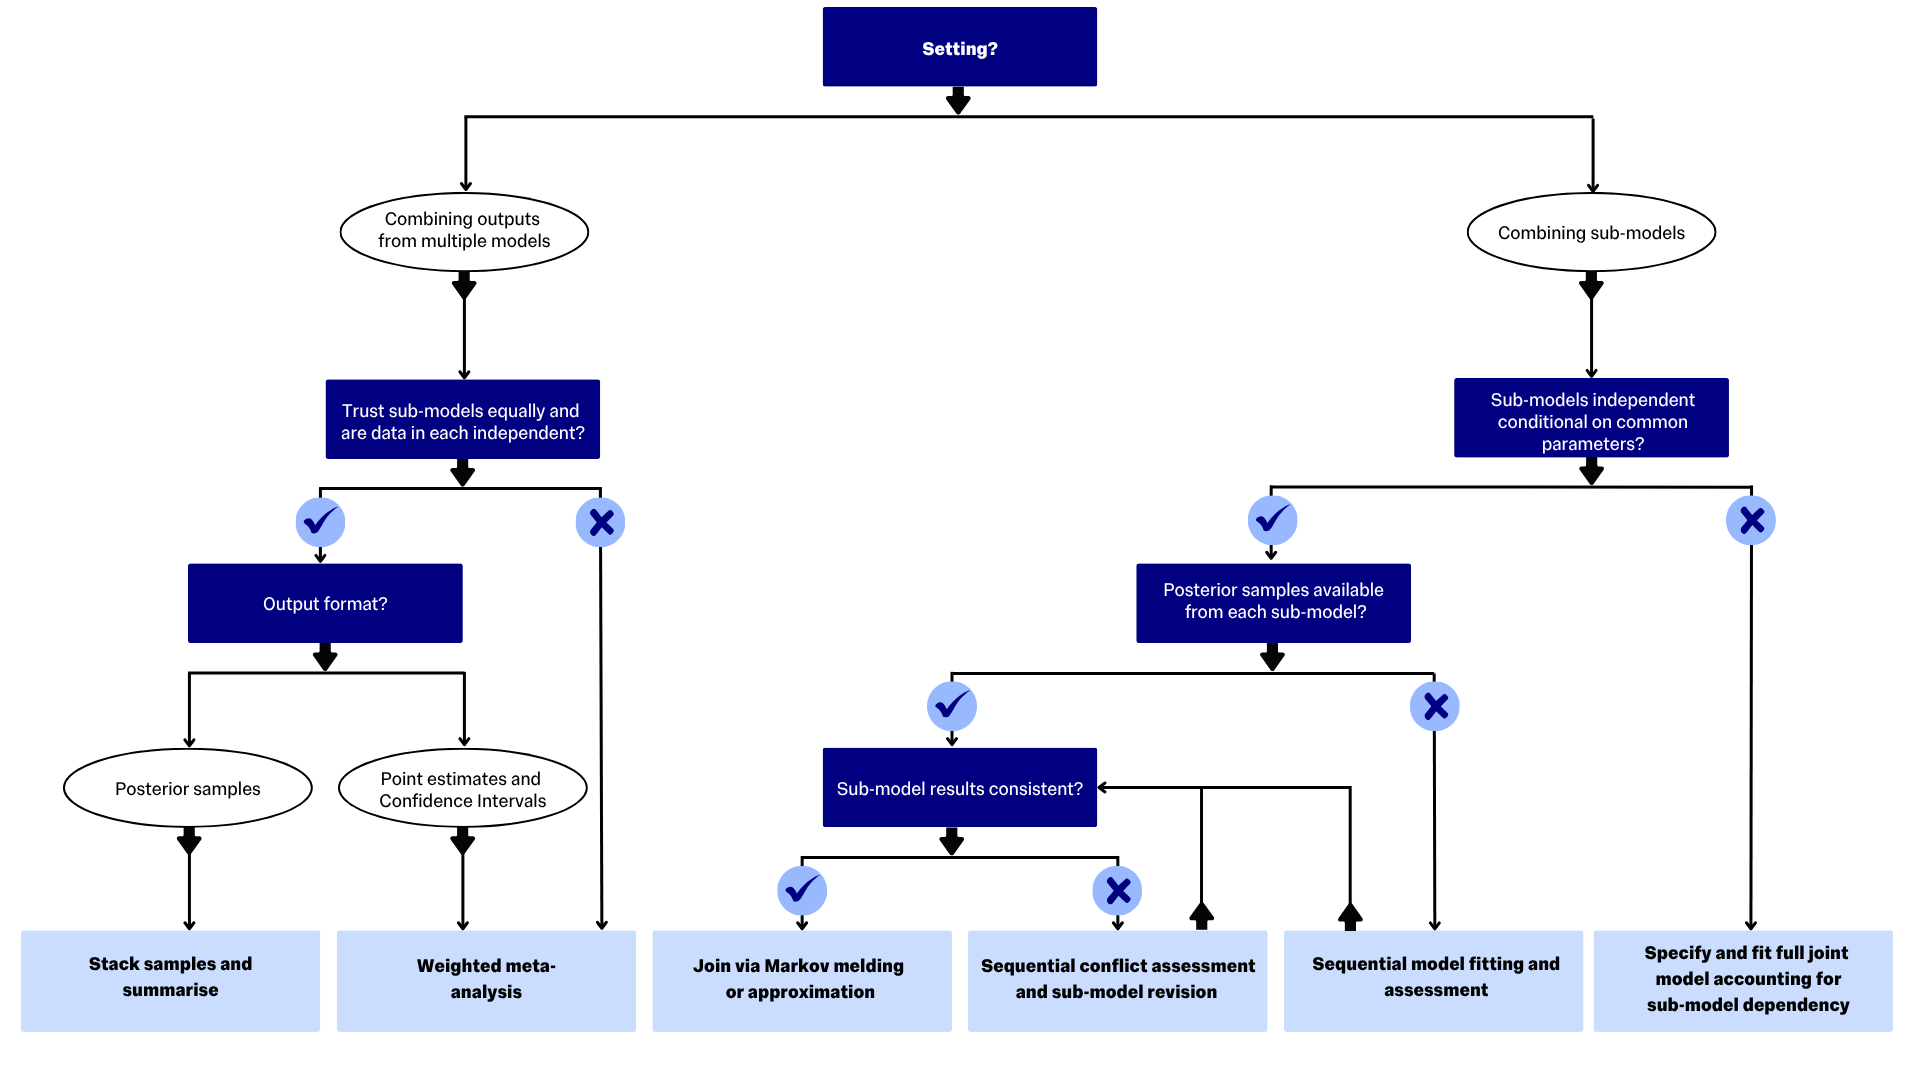
\includegraphics[width=\textwidth]{figures/Abbott et al figure 4.png}
    \caption{\textbf{Example decision tree for integration choices when integrating multiple data sources in infectious disease model inference.} Decisions depend on whether: we are combining outputs or sub-models; we trust models equally or sub-model results are consistent; format of outputs; and dependence or not of data underlying each model/sub-model. For example, if we are combining outputs and the data in each model are not independent, standard meta-analysis would overstate the certainty of estimates due to multiple use of the same data, so we might want to downweight individual models to compensate for the overconfidence.}
    \label{fig:integration}
\end{figure}

\section{Workflow Management}

\subsection{Outbreak Evolution and Workflow Iteration}  \label{sec:outbreak}
% Lead Sam Abbott
Two types of changes during outbreaks require revisiting our suggested workflow.
First, new information emerges, for example, about pathogen characteristics, surveillance capabilities, or population dynamics that may necessitate updating model assumptions and data integration choices \citep{mccaw2023role}. Substantial new data sources may also become available, such as genomic surveillance or serological surveys; or our understanding of pathogen biology may change our process model assumptions \citep{knock2021key}. 
Second, research questions commonly evolve as outbreak priorities shift from initial detection and characterisation towards intervention evaluation and long-term planning \citep{who-mosaic-2023}, altering target estimands and, therefore, our process model structure.
When these changes occur, we recommend iterating through the workflow, revisiting earlier decisions, rather than developing entirely new models.

The modular approach we advocate enables this approach, as we can update specific workflow components whilst preserving elements from previous iterations.
For example, observation models developed for case surveillance can often be reused when adding death reporting. On the other hand, process models for transmission dynamics may require updating when new variants emerge, whereas we may be able to reuse observation processes as they are.
This incremental approach reduces development time and maintains continuity across evolving outbreak contexts.

These steps are often carried out on an ad-hoc basis by teams during outbreaks.
We think that a more formal approach that tracks decisions is likely to improve the quality of models produced and be ultimately less resource-intensive.
We recommend establishing regular review points to assess whether workflow iteration is needed, with more regular reviews during acute outbreak phases.

\subsection{Reporting} \label{sec:reporting}
% Lead Sam Abbott
We have found that complex multi-source models require clear documentation to enable evaluation and reproduction.
Without structured reporting, even well-designed workflows are challenging to assess or improve.
Reporting decisions made at each stage of the workflow is essential, including rationales for data source selection, integration method choices, model structure assumptions, and validation procedures undertaken.
Making analyses public at all stages builds trust, though confidential data requires careful management \citep{Abbott2021-delta, Abbott2022-prevalence}. 
We recommend sharing code and data alongside results because it enables verification, accelerates progress, and is just as much a part of the analysis as the manuscript.
Not sharing code, sharing it on request, or only once a paper is in a peer-reviewed journal all create barriers to assessing model development and criticism workflows.
Where barriers to transparent reporting exist, it is always better to report as much as possible.
Mathematical specifications, validation code, and synthetic examples all contribute to transparency even when data cannot be shared, e.g. helping readers understand model behaviour \citep{Mellor2025-norovirus}.
We also recommend visual schematics of the workflow and model architecture are developed and referred to throughout the reporting process.

\section{Case Studies}
\label{sec:casestudies}
% Lead: Michael Plank

We demonstrate our iterative workflow through four case study schematics, each increasing in complexity and showing different integration choices and methodological considerations. All our case studies share a common estimand -- the time-varying reproduction number ($R_t$) -- while the final case study has the overdispersion parameter ($k$) as an additional estimand.

To support these case studies, we first provide examples of our suggested data review approach (Section \ref{sec:datareview}), focusing on the data streams we use in the case studies, based on an example structured questionnaire.
The examples illustrate how the strengths and limitations of each stream are reflected in practice, including variability in factors such as resolution, data utility, and practical considerations. This characterisation shows how these features shape the suitability of each stream for integration, modelling, and inference.

The case studies illustrate progressive integration of data sources.
Case study 1 uses a single data source, reported case counts.
Case study 2 combines case data with death data, overcoming some limitations of each single source. Case study 3 adds wastewater data, which are independent of surveillance biases but have their own drawbacks and biases, as a third source. Case studies 1--3 all use aggregated data that cannot capture individual variability. Case study 4 combines case counts with individual-level transmission pair data to estimate overdispersion.

Whilst these case studies focus on discrete-time branching process and renewal equation models, there is a wide range of other infectious disease modelling approaches. Our workflow applies in these more general settings.

\subsection{Data Sources and Characteristics}

During an in-person workshop, we designed a questionnaire for evaluating data characteristics across data sources to support both qualitative and quantitative assessment (Supplementary Material S2).
As a group, we then completed the questionnaire, drawing on our collective experience modelling infectious diseases during the COVID-19 pandemic.
We characterised confirmed case notifications, deaths, transmission pairs, and wastewater data, as well as additional data sources presented in the Supplementary Material (S2). Our approach was ad hoc and is intended to be representative of the review process rather than a definitive assessment.

As suggested in our workflow, before starting to design a model in response to a research question, it is often useful to characterise the kinds of data sources that are available. Here we see that our responses varied both by individual and data sources, reflecting differences in interpretation, disciplinary background, and experience (Figure \ref{survey_responses}, Table \ref{tab:survey_results}). We saw confirmed cases and deaths as mostly serving clinical purposes (75\% and 80\% of responses), while we viewed transmission pairs and wastewater as non-clinical (100\%  responses). We thought that scope differed with 88\% of us seeing confirmed cases as targeting the whole population based on the data, compared to 80\% for deaths, 20\% for transmission pairs, and 50\% for wastewater. We also thought that stratification was common in transmission pairs (80\%) and confirmed cases (75\%), but absent in wastewater. In these example datasets, we considered data formats to range from fully individual-level (100\% for transmission pairs) to fully aggregated (100\% for wastewater). We felt that temporal data were present in all sources, but spatial resolution varied, with wastewater rated highest (100\%). For prevalence, we thought that confirmed cases were split (25\% direct, 38\% indirect, 38\% not informed), and wastewater was consistently indirect (100\%). We also thought that scalability was linear for cases (63\%), exponential for transmission pairs (60\%), and independent for wastewater (83\%). Our quantitative ratings reinforced these patterns, with deaths scoring the highest test sensitivity (mean: 4.8 [range: 4-5]), and wastewater and deaths rated lowest for linkage potential (2 [1,5] and 2[1,3], respectively). Our example responses highlight how expert assessments can diverge across contexts, even within a shared framework. The variation in our views highlights the importance of acknowledging context-specific practices when evaluating data sources.

\Fontvi{
% \usepackage{color}
% \usepackage{tabularray}
\definecolor{Alto}{rgb}{0.827,0.827,0.827}
\begin{longtblr}[
  caption = {Categorical survey responses for confirmed time series (8 responses), deaths (5 responses), transmission pairs (5 responses), and wastewater (6 responses). },
  label = {tab:survey_results},
]{
  width = \linewidth,
  colspec = {Q[112]Q[377]Q[163]Q[67]Q[123]Q[90]},
  column{3} = {c},
  column{4} = {c},
  column{5} = {c},
  column{6} = {c},
  cell{87}{2} = {c=5}{0.82\linewidth},
  hline{1,88} = {-}{0.08em},
  hline{2,87} = {-}{},
  hline{3-8,10-29,31-55,57-81,83-86} = {2-6}{Alto},
  hline{9,30,56,82} = {-}{Alto},
}
\textbf{Core characteristic} & \textbf{Characteristic} & {\textbf{Confirmed cases time series}\\N = 8\textit{\textsuperscript{1}}} & {\textbf{Deaths}\\N = 5\textit{\textsuperscript{1}}} & {\textbf{Transmission pairs}\\N = 5\textit{\textsuperscript{1}}} & {\textbf{Wastewater}\\N = 6\textit{\textsuperscript{1}}}\\
{\textbf{Basic}\\\textbf{meta-data}} & \textbf{Study design} &  &  &  & \\
 & ~~~~Contact tracing & 0\% & 0\% & 100\% & 0\%\\
 & ~~~~Routine surveillance & 88\% & 100\% & 0\% & 50\%\\
 & ~~~~Sentinel surveillance & 13\% & 0\% & 0\% & 50\%\\
 & \textbf{Primary purpose} &  &  &  & \\
 & ~~~~Clinical management & 75\% & 80\% & 0\% & 0\%\\
 & ~~~~Other & 25\% & 20\% & 100\% & 100\%\\
\textbf{Scope} & \textbf{Target population} &  &  &  & \\
 & ~~~~Convenience & 0\% & 0\% & 20\% & 0\%\\
 & ~~~~Geographic structure & 13\% & 0\% & 0\% & 50\%\\
 & ~~~~Geographic structure, Whole population & 0\% & 20\% & 0\% & 0\%\\
 & ~~~~Healthcare workers & 0\% & 0\% & 20\% & 0\%\\
 & ~~~~Risk-specific & 0\% & 0\% & 20\% & 0\%\\
 & ~~~~Specific age groups, Risk-specific, Convenience & 0\% & 0\% & 20\% & 0\%\\
 & ~~~~Whole population & 88\% & 80\% & 20\% & 50\%\\
 & \textbf{Stratification} &  &  &  & \\
 & ~~~~Clinical & 0\% & 0\% & 40\% & 0\%\\
 & ~~~~Demographic & 38\% & 40\% & 20\% & 0\%\\
 & ~~~~Demographic, Clinical & 38\% & 20\% & 40\% & 0\%\\
 & ~~~~None & 25\% & 40\% & 0\% & 100\%\\
 & \textbf{Collection type} &  &  &  & \\
 & ~~~~One-off & 0\% & 0\% & 20\% & 0\%\\
 & ~~~~Routine & 100\% & 100\% & 0\% & 100\%\\
 & ~~~~Triggered & 0\% & 0\% & 80\% & 0\%\\
 & \textbf{If triggered, potential triggers} &  &  &  & \\
 & ~~~~Greater than a threshold & 0\% & 100\% & 0\% & NA\\
 & ~~~~New variant/pathogen detected & 100\% & 0\% & 100\% & NA\\
 & ~~~~Unknown & 7 & 4 & 1 & 6\\
\textbf{Resolution} & \textbf{Data aggregation} &  &  &  & \\
 & ~~~~Aggregated & 50\% & 60\% & 0\% & 100\%\\
 & ~~~~Individual & 50\% & 40\% & 100\% & 0\%\\
 & \textbf{Temporal data} &  &  &  & \\
 & ~~~~Yes & 100\% & 100\% & 100\% & 100\%\\
 & \textbf{Collection frequency} &  &  &  & \\
 & ~~~~Continuously & 25\% & 40\% & 60\% & 17\%\\
 & ~~~~Daily & 63\% & 60\% & 20\% & 0\%\\
 & ~~~~Multiple times a week & 0\% & 0\% & 20\% & 67\%\\
 & ~~~~Weekly & 13\% & 0\% & 0\% & 17\%\\
 & \textbf{Reporting frequency} &  &  &  & \\
 & ~~~~Continuously & 0\% & 0\% & 20\% & 0\%\\
 & ~~~~Daily & 50\% & 40\% & 40\% & 0\%\\
 & ~~~~Less frequently than monthly & 0\% & 0\% & 20\% & 0\%\\
 & ~~~~Multiple times a week & 0\% & 0\% & 20\% & 33\%\\
 & ~~~~Weekly & 50\% & 60\% & 0\% & 67\%\\
 & \textbf{Time period covered} &  &  &  & \\
 & ~~~~Continuous & 88\% & 100\% & 0\% & 83\%\\
 & ~~~~Early outbreak & 0\% & 0\% & 100\% & 0\%\\
 & ~~~~Endemic & 13\% & 0\% & 0\% & 17\%\\
 & \textbf{Spatial data} & 63\% & 80\% & 80\% & 100\%\\
 & \textbf{Spatial resolution} &  &  &  & \\
 & ~~~~Hyper-local & 0\% & 0\% & 40\% & 0\%\\
 & ~~~~Local & 13\% & 40\% & 40\% & 100\%\\
 & ~~~~National & 25\% & 20\% & 0\% & 0\%\\
 & ~~~~Regional & 63\% & 40\% & 20\% & 0\%\\
\textbf{Data utility} & \textbf{Quantities informed [Basic reproduction number]} &  &  &  & \\
 & ~~~~Direct & 0\% & 0\% & 0\% & 17\%\\
 & ~~~~Direct, Indirect & 0\% & 20\% & 20\% & 0\%\\
 & ~~~~Indirect & 88\% & 80\% & 80\% & 17\%\\
 & ~~~~Not informed & 13\% & 0\% & 0\% & 67\%\\
 & \textbf{Quantities informed [Time-varying reproduction number]} &  &  &  & \\
 & ~~~~Direct & 50\% & 0\% & 0\% & 17\%\\
 & ~~~~Indirect & 50\% & 100\% & 100\% & 83\%\\
 & \textbf{Quantities informed [Time-varying / basic reproduction number ratio]} &  &  &  & \\
 & ~~~~Direct & 0\% & 0\% & 0\% & 17\%\\
 & ~~~~Indirect & 88\% & 100\% & 100\% & 17\%\\
 & ~~~~Not informed & 13\% & 0\% & 0\% & 67\%\\
 & \textbf{Quantities informed [Incidence]} &  &  &  & \\
 & ~~~~Direct & 50\% & 0\% & 0\% & 0\%\\
 & ~~~~Indirect & 50\% & 100\% & 80\% & 67\%\\
 & ~~~~Not informed & 0\% & 0\% & 20\% & 33\%\\
 & \textbf{Quantities informed [Prevalence]} &  &  &  & \\
 & ~~~~Direct & 25\% & 0\% & 0\% & 0\%\\
 & ~~~~Indirect & 38\% & 80\% & 80\% & 100\%\\
 & ~~~~Not informed & 38\% & 20\% & 20\% & 0\%\\
 & \textbf{Quantities informed [Heterogeneity in transmission (e.g. superspreading)]} &  &  &  & \\
 & ~~~~Indirect & 50\% & 40\% & 100\% & 0\%\\
 & ~~~~Not informed & 50\% & 60\% & 0\% & 100\%\\
 & \textbf{Quantities informed [Drivers of transmission]} &  &  &  & \\
 & ~~~~Indirect & 38\% & 40\% & 100\% & 0\%\\
 & ~~~~Not informed & 63\% & 60\% & 0\% & 100\%\\
{\textbf{Practical~}\\\textbf{considerations}} & \textbf{Scalability} &  &  &  & \\
 & ~~~~Exponentially & 0\% & 20\% & 60\% & 0\%\\
 & ~~~~independent & 0\% & 20\% & 0\% & 83\%\\
 & ~~~~Linearly & 63\% & 60\% & 40\% & 0\%\\
 & ~~~~Sub-exponentially & 38\% & 0\% & 0\% & 17\%\\
 & \textit{\textsuperscript{1}}~\% &  &  &  & 
\end{longtblr}
}

\begin{figure}[H] 
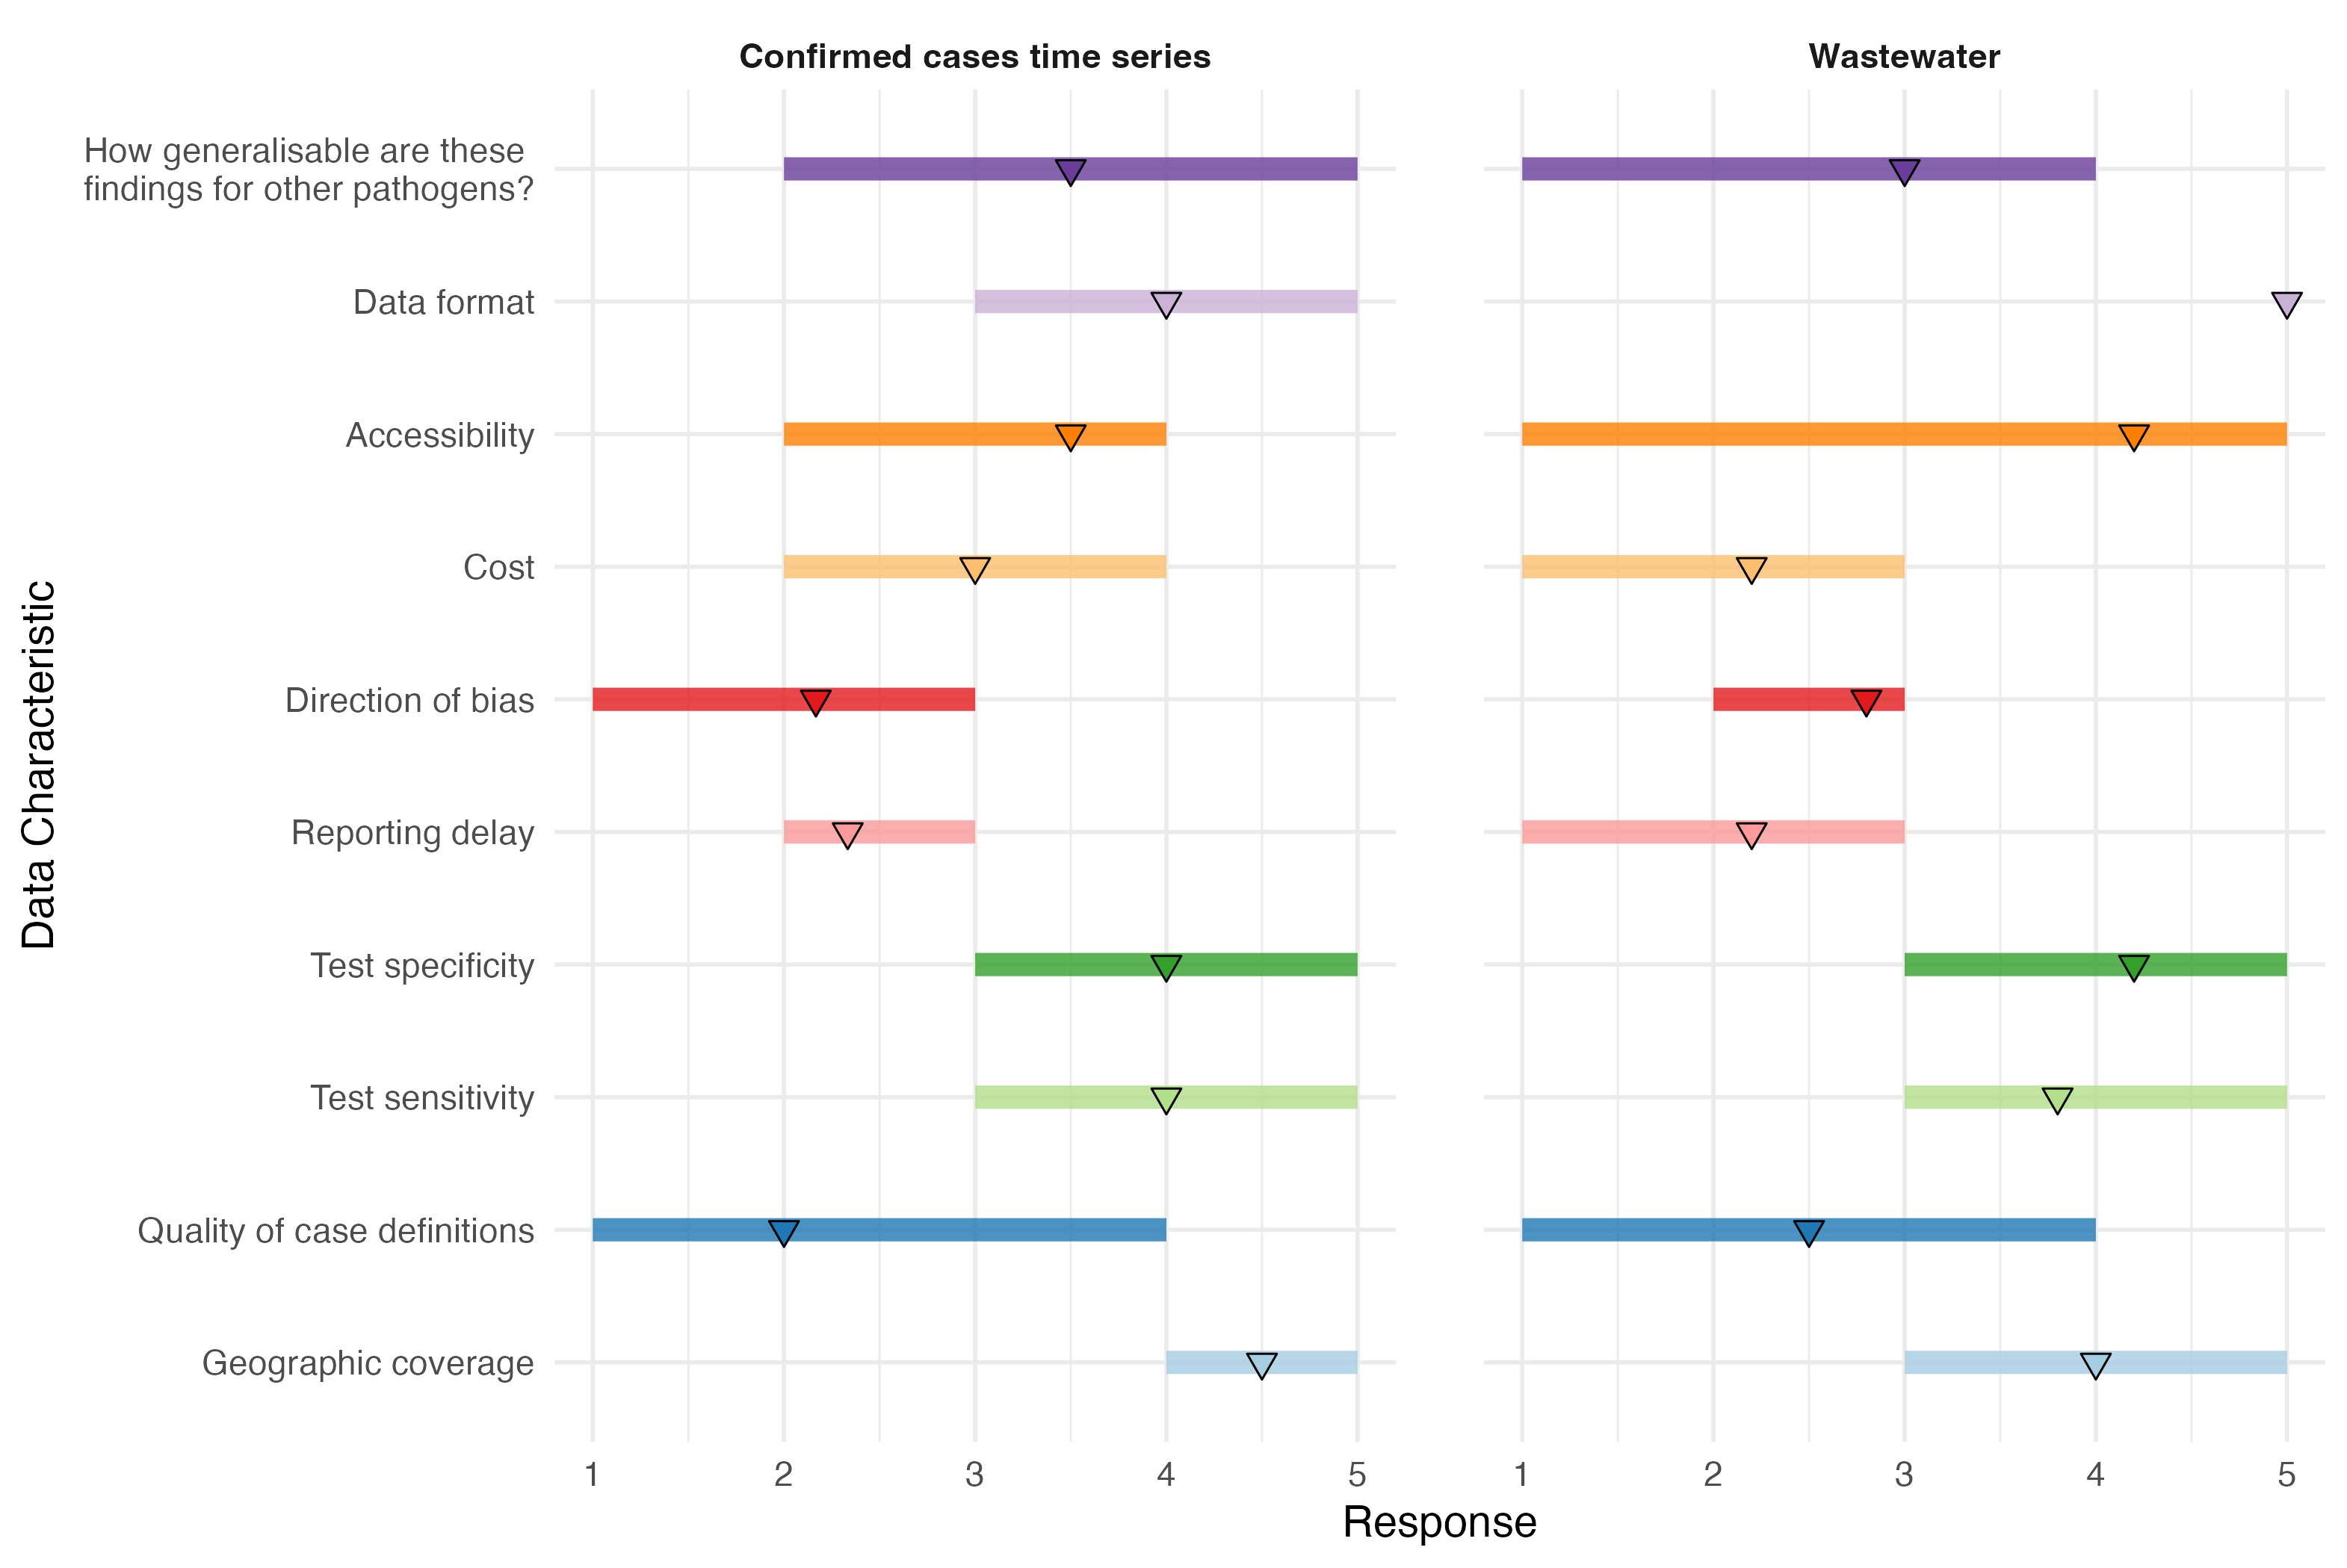
\includegraphics[width=1\linewidth]{figures/survey_responses.png}
\centering
\caption{ Selected data characteristics from the survey, showing responses related to confirmed case time series (8 responses), deaths (5 responses), transmission pairs (5 responses), and wastewater surveillance (6 responses). The y-axis represents specific data characteristics, while the x-axis indicates the response range on a 5-point scale, where 1 corresponds to a low level and 5 to a high level. The lower triangles present the average response for each data characteristic.}
\label{survey_responses}
\end{figure}



\subsection{Case Study 1: Single-Source Baseline (Cases Only)}


In this case study, we showcase our workflow by exploring some of the assumptions and modelling and fitting choices underlying the estimation of $R_t$ from a single time series of case incidence.

\textbf{Workflow Demonstration:}
\begin{enumerate}
    \item \textbf{Research question and target estimands:} The research question for this case study (and case studies 2 and 3) is: What is the time-varying reproduction number $R_t$ during this outbreak period?

    \item \textbf{Process DAG development:} We choose to use a discrete-time model with a daily time step. This is convenient as it matches the frequency of reported data in many real-world surveillance systems. However, we note that other choices are possible, including continuous-time models or different choices of time step. Also, it is not necessary for the time step in the process model to be the same as the data reporting frequency and it is possible to explicitly model the temporal aggregation of transmission events observed with interval censoring as part of the observation model. We begin with a flexible branching process model for the number of people $N_{i,t}$ newly infected by individual $i$ on day $t$:
    \begin{equation} \label{eq:individual_level}
         N_{i,t} \sim \mathrm{Poiss} \left( Y_i R_t g_{t-T_i} \right)
    \end{equation} 
    Here, $T_i$ is the infection time of individual $i$, $Y_i$ is the relative transmission rate of individual $i$ (which may capture a combination of biological and social factors), and $g_s$ is the relative infectiousness $s$ days after infection normalised such that $\sum_{s=1}^\infty g_s=1$. We start with this approach as it explicitly models the full transmission tree of the epidemic whilst remaining relatively parsimonious. We further assume that the infectiousness profile $g_s$ does not change over time, but note that we would need to revisit this assumption if there was evidence this had changed, for example due to biological changes in the pathogen, changes in contact patterns, or case isolation measures. The daily infection incidence $I_t=\sum_i N_{i,t}$ satisfies
    \begin{equation} \label{eq:It_with_hetergoeneity}
        I_t \sim \mathrm{Poiss}\left( R_t \sum_i Y_i g_{t-T_i} \right)
    \end{equation}


\item \textbf{Data source selection:} Case incidence data is typically readily available with very frequent updates and relatively good timeliness (good scope and resolution), though this can depend on lab processing and reporting timelines. These factors make case data an obvious choice for trying to model time-varying transmission parameters. However, case counts are an imperfect and often biased proxy for infection incidence and are sensitive to testing patterns, which can vary over time (data quality issues) -- see Table \ref{tab:survey_results} and Figure \ref{survey_responses}. 


\item \textbf{Observation DAG construction:} The observation model relates the observed data (here daily case incidence) with underlying latent variables (here, daily infection incidence). 
This requires us to make assumptions about case ascertainment (what fraction of infections are detected cases), reporting delays (time between infection and a case being detected and reported), and random noise (typically used to capture other things not explicitly specified in the model).

There are at least  $2^3=8$ possible observation models to consider, which either ignore or include each of these three aspects.
We refer to these models as $O_{000}$ (for the simplest observation model not modelling any of the above) to $O_{111}$ (for the most comprehensive accounting for all three observation features). We represent the $O_{111}$ model by the following equation for the observed variable $C_t$, representing the number of reported cases on day $t$:
\begin{equation} \label{eq:cases}
    C_t \sim \mathrm{Poiss}\left( \sum_{s=1}^t M_{t-s,s}\right)
\end{equation}
where $M_{t,s}$ is the number of people infected on day $t$ and reported as a case $s$ days later, given by
\begin{equation}
    M_{t,.} \sim \mathrm{TruncatedMultinomial}\left( I_t, p_c \boldsymbol{\alpha} \right) 
\end{equation}
Here $p_c$ is the probability an infection is reported as a case (i.e. case ascertainment ratio), which we assume to be constant over time, and $\boldsymbol{\alpha}$ is a vector containing the probability mass function of the distribution of time from infection to reporting. We choose to use the most comprehensive observation model $O_{111}$ as it is generally important to account for all three factors.



\item \textbf{Refine the model DAGs:} Since we only have aggregate-level data on the number of reported cases and no individual-level data about the transmission tree, and no explicit domain knowledge to inform a prior, we recognise that individual heterogeneity in transmission rates (represented by the variable $Y_i$) will not be identifiable. We therefore simplify the model by assuming that $Y_i=1$ for all individuals. With this simplification, Eq. \eqref{eq:It_with_hetergoeneity} for daily infection incidence $I_t$ reduces to
    \begin{equation} 
        I_t \sim \mathrm{Poiss}\left( R_t \sum_{s=1}^\infty I_{t-s}g_s  \right)
    \end{equation}
    This is an example of the well-known renewal process model \cite{fraser2007estimating}. This is a popular model for $R_t$ estimation as it captures fundamental features of the transmission process (newly infected individuals at time $t$ transmit the pathogen to other individuals some time later), without making additional assumptions, for example, about the size of the susceptible population or the strength and duration of infection-acquired immunity. This provides a simple but flexible model to which additional complexity can be added in subsequent iterations of the workflow.
    There are other valid assumptions we might wish to make depending on other workflow considerations. Here, we consider three variants of the renewal process model, which, conditional on previous infections, all have the same mean daily infection incidence $E(I_t)$, but assume different models for the distribution of $I_t$:
    \begin{itemize}
    \item[$P_1$.] Deterministic model for daily infection incidence (no variance).
    \begin{equation} \label{eq:infections_P1}
        I_t = R_t \sum_{s=1}^\infty I_{t-s}g_s 
    \end{equation}
    \item[$P_2$.] Poisson-distributed daily infection incidence.
        \begin{equation} \label{eq:infections_P2}
        I_t \sim \mathrm{Poiss}\left( R_t \sum_{s=1}^\infty I_{t-s}g_s  \right)
    \end{equation}
    \item[$P_3$.] Negative binomially distributed daily infection incidence (larger variance than Poisson). 
            \begin{equation} \label{eq:infections_P3}
        I_t \sim \mathrm{NegBin}\left( R_t \sum_{s=1}^\infty I_{t-s}g_s, k  \right)
    \end{equation}
    where $k$ is the dispersion parameter. 
    \end{itemize} 
Figure \ref{fig:case_study_visual} shows the process \ac{DAG}s and observation \ac{DAG}s for all potential models. Here, $P_1$ is unlikely to be realistic as there will almost always be some source of random variability in daily infection incidence. The choice between $P_2$ and $P_3$ could depend on whether superspreading is known to be a major factor in the transmission dynamics. Since $P_3$ contains $P_2$ in the limiting case $k\to\infty$, we choose to use $P_3$ in this example (see Figure \ref{fig:case_study_diagram}).
Importantly, the negative binomial distribution in $P_3$ captures both potential biological overdispersion (superspreading) and unmodelled variance in the data. We could include additional sources of noise in the observation model (e.g. day-of-the-week reporting effects \citep{abbott2020estimating}) if the data showed evidence for these either on first inspection or during model specification and validation.


\item \textbf{Modularise the DAGs:} Here, we do not need to do any modularisation as we are only dealing with a single data source, and the model is simple enough that we don't need to investigate the process and observation models as separate modules.

\item \textbf{Inference and implementation choices:} Implementation now requires selection of one process model, one observation model and one fitting method. The choice of fitting method depends on the analytical tractability of the combined process and observation model, computational complexity and speed of computation relative to the time available, and identifiability issues (see Section \ref{sec:fitting}). 
For our chosen combination of models ($P_3$-$O_{111}$), we recommend using \ac{NUTS}, but only if we can approximate the discrete observation models (e.g. EpiNow2 \citep{abbott2020estimating}). If approximation is not feasible or warranted, we would need to use an alternative method such as \ac{PMCMC}. If we needed a simpler, more computationally efficient fitting method, we could return to the ``Refine models'' stage and select a simpler model. For the simplest model combination with no underreporting, delays or observation noise ($P_1$-$O_{000}$), we can calculate $R_t$ directly for a given choice of generation time distribution by rearranging Eq. \eqref{eq:infections_P1}. This is likely to give biased and highly noisy estimates in practice and does not provide any uncertainty quantification. For the next-simplest model ($P_2$-$O_{000}$), we can calculate an analytical posterior distribution for $R_t$  from a conjugate gamma prior, which is fast and computationally efficient. This is implemented in the widely used EpiEstim method \citep{cori2013new}. 

\item \textbf{Model specification and validation:} Model specification requires a prior for $R_t$ as well as specification of the profile of infectiousness over time $g_t$, the reporting probability $p_c$, the distribution of time from infection to reporting $\boldsymbol{\alpha}$ and (for process model $P_3$) the dispersion coefficient $k$. The simplest approach is to take these as fixed parameters, which corresponds to an infinite-strength prior. This is unlikely to ever be appropriate but may be required for computational tractability. However, a better approach in the presence of uncertainty is to define a prior over these parameters based on domain expertise. In the case of probability distributions ${\bf g}$ and $\boldsymbol{\alpha}$, we could use a parametric distribution assumption, e.g. a discretised gamma \citep{charniga2024best,park2024estimating} or other non-negative-integer valued distribution with specified priors for the mean and variance. 

Different modelling approaches have different strengths and limitations. For example, simple approaches are fast to implement, but ignore important factors in the data observation process. These may be useful for a quick initial estimate, but should be revisited as needed. In this case study, $R_t$ estimates may be insensitive to underreporting provided the reporting fraction is constant over the period of interest. Furthermore, any change in reporting fraction will not be identifiable from a case time series alone (if $R_t$ varies over the same time scale), so it would not be sensible to attempt to estimate a time-varying reporting fraction in this example. However, reporting delays can be substantial and will affect both the magnitude and timing of $R_t$ estimates. We can account for this effect by selecting an appropriate observation model, at the cost of needing to move to a more computationally costly fitting method. Ultimately, the most appropriate option will depend on the balance between need for timely estimates (e.g. for modelling an outbreak in real-time) and the realism of the associated assumptions. 
Finally, a common weakness of all the models outlined above is that they assume the profile of infectiousness over time is constant. Some approaches (e.g. some versions of EpiEstim, and EpiNow2 \citep{abbott2020estimating}) extend the approach to relax this assumption.
 
\item \textbf{Data integration choices:} As there is only one data source in this case study, we do not need to make any decisions about what and how to integrate multiple sources. In a scenario where multiple groups use different methods to produce estimates of the target estimand (in this case $R_t$) based on the same data, we could integrate the results by ensembling them into a combined estimate \citep{maishman2022statistical,manley2024combining}. In this context, it is desirable to align the assumptions made by different models, for example, about the generation time distribution or the temporal smoothness in $R_t$, to ensure that estimates from the different models are comparable \citep{brockhaus2023why}. Potentially, estimates may also need to be downweighted when drawn from the same data sources.

 \end{enumerate}
 


\begin{figure}[htbp]
    \centering
    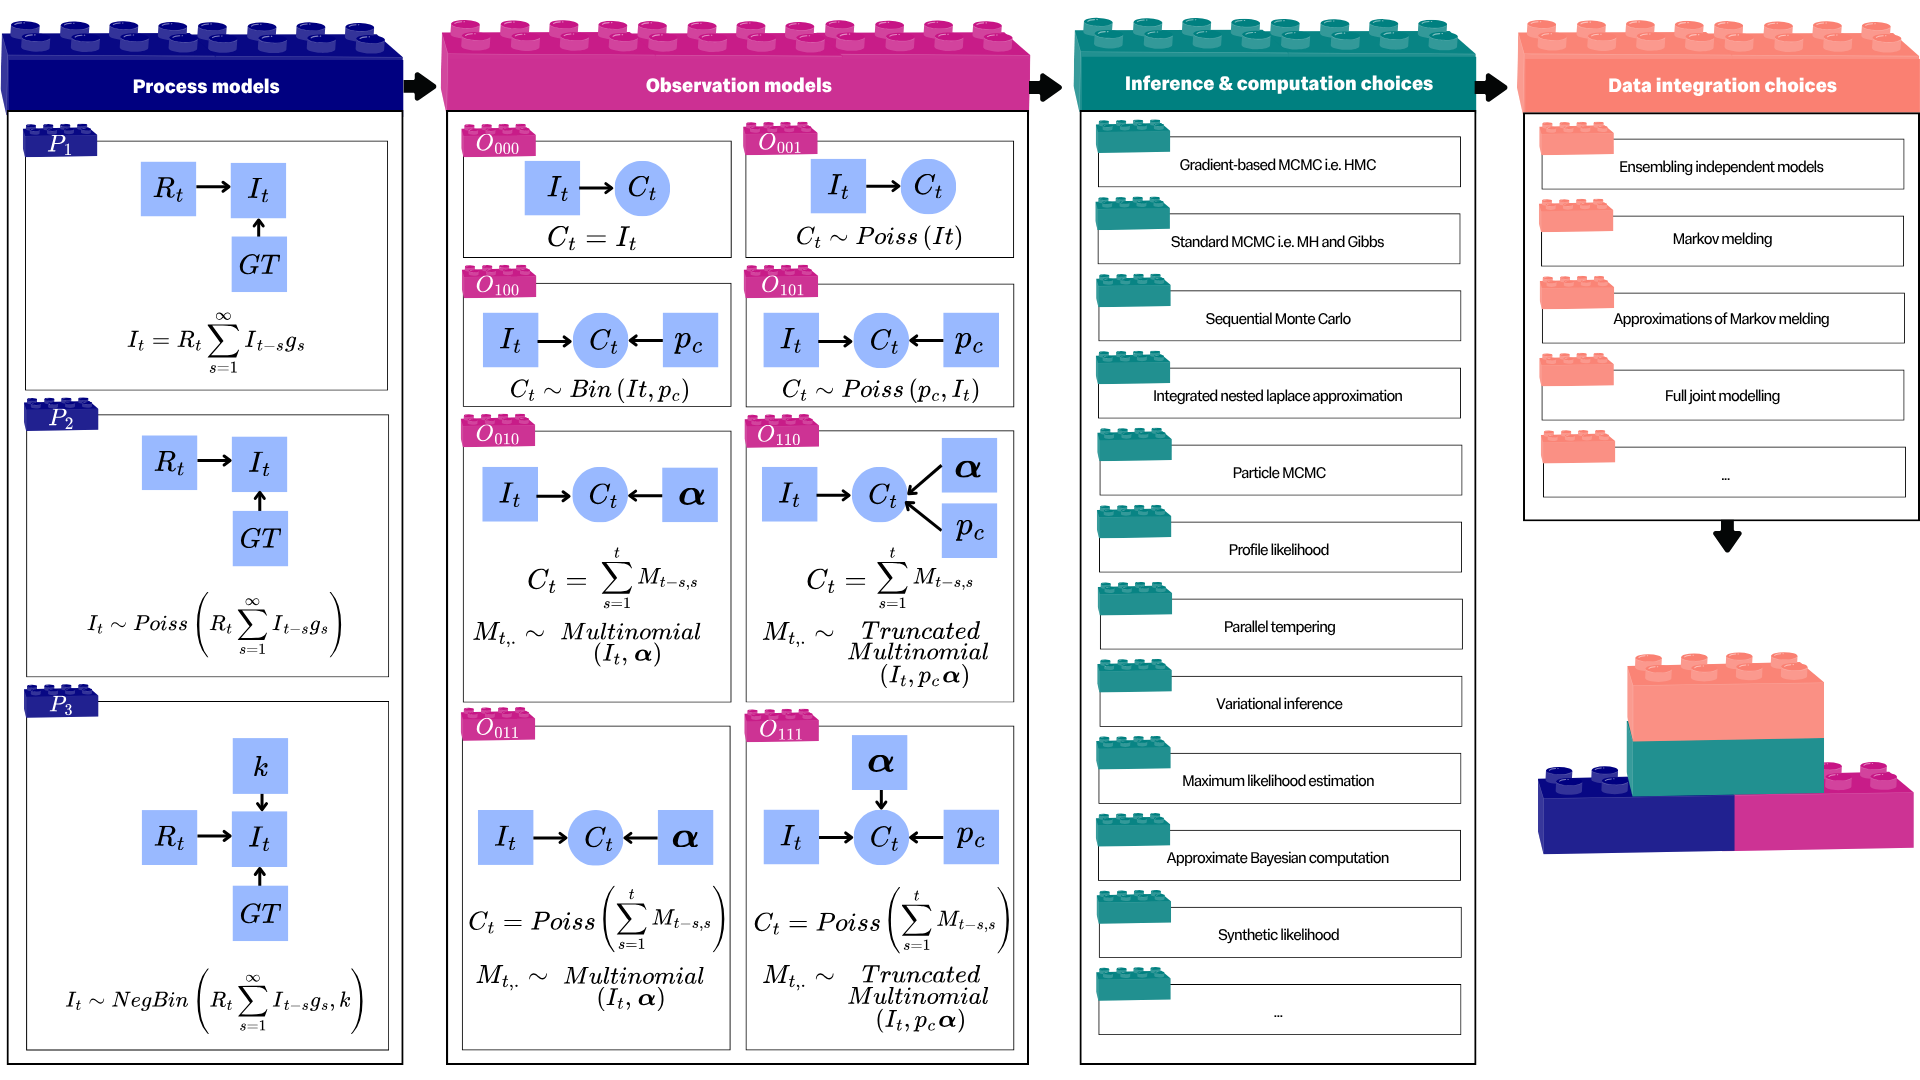
\includegraphics[width=\textwidth]{figures/Abbott et al figure 6.png}
    \caption{\textbf{Modular representation for infectious disease modelling showing the interchangeable components of process models, observation models, integration approaches, and fitting methods.} Process models include deterministic ($P_1$), stochastic Poisson ($P_2$), and negative binomial ($P_3$) formulations relating reproduction number ($R_t$) to number of new infections ($I_t$) with generation time ($GT$) distributions. $P_3$ incorporates overdispersion parameter $k$ to caption extra-Poisson variation. Observation models range from direct observation ($O_{000}$) to complex hierarchical structures ($O_{111}$) that model the relationship between $I_t$ and (observed) case incidence through underreporting, reporting delays and measurement uncertainty. The jigsaw puzzle metaphor illustrates how different modelling components can be combined flexibly, with inference method including \ac{MCMC}, \ac{VI}, \ac{ABC}, etc. Integration approaches span from full joint modelling to ensembling independent models, enabling researchers to select optimal combinations based on data availability and research objectives. }
    \label{fig:case_study_visual}
\end{figure}


\subsection{Case Study 2: Two-Source Integration (Cases and Deaths)}

More data sources often become available later in an outbreak. For example, early in an outbreak, surveillance data may be restricted to reported cases due to the delay from infection to development of clinically severe disease. However, once the outbreak has progressed and/or reporting systems are brought online, other events such as hospitalisation, \ac{ICU} admission or death notification become available. In this case study, we model time-varying transmission rates using two data sources: reported cases and deaths. We illustrate the process and challenges of adding an additional data stream and explore how this can improve $R_t$ estimation and reduce assumption dependence.

\begin{enumerate}
   \item \textbf{Research question and target estimands:}  In this case study, we target the same estimand as in case study 1 ($R_t$). 
   
    \item \textbf{Process DAG development:} We consider the same process \ac{DAG} as in case study 1 (see Figure \ref{fig:case_study_diagram}), as we assume that the addition of data on deaths does not impact the transmission process.
        
    \item \textbf{Data source selection:} Data on deaths typically have longer delays (delay from infection to death and potentially from date of death to date of registration) and are less representative of the overall population, but have lower noise (e.g. due to ``day-of-the-week'' reporting effects), higher ascertainment, and less dependence on testing patterns than case incidence data. Combining death data with case data can therefore potentially overcome some of the limitations present in each single data source. Based on the data survey (Table \ref{survey_responses}), we expect these data sources to have differing time-varying biases and so to be useful for unpicking the dynamics of the underlying infection time series. As noted, the major issue we need to be aware of is the potential for conflict as these data sets represent different target populations.
    
    \item \textbf{Observation DAG construction:} Similar to the number of reported cases defined by Eq. \eqref{eq:cases}, the number of deaths $D_t$ that occur on day $t$ depends on the time series of infections up to day $t$, the infection-fatality ratio $p_d$, and the distribution $v_s$ of time ($s$) from infection to death. We represent this in the observation \ac{DAG} (Figure \ref{fig:case_study_diagram}) and by the following convolution equation \citep{bhatt2023semi}:
    \begin{equation} \label{eq:deaths}
        D_t \sim \mathrm{Poiss}\left(p_d \sum_{s=1}^\infty I_{t-s}v_s \right)
    \end{equation}
    Other models for deaths are possible, for example, using a multinomial model for the number of deaths occurring on day $t$ due to infections on day $t-s$ ($s=1,2,\ldots$). However, the Poisson model is a good approximation provided $p_d\ll 1$. 
    Eq. \eqref{eq:deaths} provides a model for the time series of daily deaths $D_t$ conditional on the time series of daily infections $I_t$ and would be coupled with one of Eqs. \eqref{eq:infections_P1}--\eqref{eq:infections_P3}, which describe the dynamics of infections, to produce a joint model for infections and deaths. We begin with the simplest observation model, which assumes that all deaths are recorded immediately, so the observed variable is simply $D^\mathrm{obs}_t=D_t$.
    


\item \textbf{Refine the model DAGs:}       
    Similar to the different choices of observation model for cases, the observation model for deaths could include underreporting, reporting delays, and random noise. The observation model described above corresponds to $O_{000}$. However, in revisiting the data on deaths, we discover that there is sometimes a substantial delay from date of death to date of registration \citep{seaman2022nowcasting}. If we were conducting the analysis retrospectively, we could use model $O_{000}$ for data by date of death (i.e. define $D^\mathrm{obs}_t$ to be the number of deaths that occurred on day $t$). However, for a real-time analysis, this data would be incomplete and it would be important to account for the delay. Hence, we use data by date of registration (i.e. define $D^\mathrm{obs}_t$ to be the number of deaths registered on day $t$) and use model $O_{010}$. This still assumes that all deaths are eventually reported with no additional observation noise (which is reasonable for jurisdictions with comprehensive death records), but accounts for the observation delay via the following equation for the number of deaths registered on day $t$:
\begin{equation}
    D^\mathrm{obs}_t = \sum_{s=0}^\infty M_{t-s,s}
\end{equation}
where $M_{t,s}$ is the number of deaths that occurred on day $t$ and were registered $s$ days later, given by
\begin{equation}
    M_{t,.} \sim \mathrm{Multinomial}\left( D_t, \boldsymbol{\beta}\right) 
\end{equation}
where $\boldsymbol{\beta}$ is a vector containing the probability mass function for the number of days from date of death to date of registration.

 \item \textbf{Modularise the DAGs:} The module for reported cases is the same as in case study 1. Here, we add a second module for deaths (see Figure \ref{fig:case_study_diagram}).

\item \textbf{Inference and implementation choices:} As each submodel and the joint model have a differentiable likelihood, we recommend \ac{NUTS} for fitting. If some of the submodels had non-differentiable likelihoods, we would recommend using \ac{NUTS} on the submodels where this was possible, and \ac{PMCMC} on the remaining submodels and the joint model.

\item \textbf{Model specification and validation:} In addition to the parameters from case study 1, this model requires us to specify the infection fatality ratio $p_d$, the distribution of time from infection to death $\bf{v}$ and from date of death to date to date of registration $\boldsymbol{\beta}$. Again, we recommend using appropriately informative priors based on domain knowledge where possible to allow for appropriate uncertainty. 


    \item \textbf{Data integration choice:} 
       Two different approaches are possible for integration: (1) a joint model including both cases and deaths with a shared latent state $R_t$ \citep{scott2020epidemia}; (2) separate models for cases and deaths, resulting in two estimates for $R_t$ to be combined via a weighted ensemble or Markov melding.
        As outlined above, we recommend fitting separate models to the two time series initially, to understand their behaviour and reveal whether they lead to consistent or conflicting estimates of $R_t$ \citep{sherratt2021exploring}. Inconsistent results emerging from the two data sources could prompt us to refine the model. For example, if $R_t$ estimates show similar trends but shifted in time, we would need to revisit assumptions about delays (return to model specification and validation (Section~\ref{sec:spec-validate})). If $R_t$ estimates are largely consistent, but the case-based estimate shows a transient increase in $R_t$ that does not occur in the deaths-based estimate, an increase in case ascertainment might be an explanation (return to refine the model \ac{DAG}s (Section~\ref{sec:refine-dags}) to include time-varying ascertainment). In case study 1, using data on cases alone, the case ascertainment ratio was non-identifiable and had to be assumed. Including data on deaths allows estimation of trends in case ascertainment, provided the infection-fatality ratio can be assumed constant over time. If the infection-fatality ratio additionally has a relatively informed prior distribution, the absolute value of case ascertainment can be estimated. Both approaches require assumptions about the distribution of time from infection to death, demonstrating how additional data sources can shift rather than eliminate the need for modelling assumptions. As both of these models are relatively simple Markov melding is likely not needed when fitting the joint model.
\end{enumerate}

\subsection{Case Study 3: Three-Source Integration (Cases, Deaths and Wastewater)}

Wastewater-based epidemiology has emerged as a complementary data source to traditional disease surveillance methods \citep{keshaviah2023wastewater}. Wastewater surveillance has been used for a range of viral pathogens including norovirus \citep{zheng2024tracking}, poliovirus \citep{whitehouse2024wastewater}, and influenza viruses \citep{zheng2023development}. During the Covid-19 pandemic, wastewater surveillance supported outbreak detection \citep{hewitt2022sensitivity}, situational awareness and forecasting \citep{varkila2023use,jin2024combining}, and multi-strain modelling \citep{dreifuss2025estimated}. 

\begin{enumerate}
   \item \textbf{Research question and target estimands:} In this case study, we include measurements of viral \ac{RNA}/\ac{DNA} concentration in wastewater samples as a third data source alongside reported cases and deaths. We explore ways of handling conflicting signals between data sources and incorporating complex observation processes. The target estimand is $R_t$, as in case studies 1 and 2.
   
    \item \textbf{Process DAG development:} We start with the same process \ac{DAG} as in case studies 1 and 2 (see Figure \ref{fig:case_study_diagram}).

    \item \textbf{Data source selection:} Wastewater data offers population-level information (broad scope) independent of testing biases and changes in testing rates, with moderate timeliness, but requires environmental expertise and is subject to high levels of unexplained variability. It could also be sensitive to unknown changes in the average shedding rate over time and, often, has relatively poor resolution (limited spatial resolution and no information about age or other demographic variables). 

    
    \item \textbf{Observation DAG construction:} 
    Suppose that the average viral \ac{RNA}/\ac{DNA} load $W_t$ in wastewater on day $t$, typically quantified in genome copies per person per day, depends on the time series of infections up to day $t$ and the average amount of viral \ac{RNA}/\ac{DNA} that an individual sheds into wastewater $s$ days after being infected ($s=1,2,\ldots$). We represent this in the process \ac{DAG} in Figure \ref{fig:case_study_diagram} and the following equation for $W_t$:
    \begin{equation} \label{eq:wastewater}
        W_t = \frac{c}{N_\mathrm{pop}}\sum_{s=1}^\infty I_{t-s}u_s 
    \end{equation}
    where $c>0$ is a constant representing the average total amount of viral \ac{RNA}/\ac{DNA} that an infected individual sheds over the course of their infection, $N_\mathrm{pop}$ is the total population size, and $u_s$ is the average shedding rate $s$ days after infection, normalised such that $\sum_{s=1}^\infty u_s=1$. We would couple Eq. \eqref{eq:wastewater} with one of Eqs. \eqref{eq:infections_P1}--\eqref{eq:infections_P3} for infections.
    
   Wastewater samples are typically collected at some cadence from one or more sampling sites, and the concentration of viral \ac{RNA}/\ac{DNA} in the samples is quantified via \ac{PCR} testing. The existence of multiple sites with different catchment populations and non-contemporaneous sampling frequencies complicates the interpretation of quantitative wastewater data, which can be modelled at varying levels of complexity.   
   Suppose that measurements of the wastewater concentration $W^\mathrm{obs}_{j,t}$ are taken from sampling sites $j=1,\ldots, J$ on some subset of days $t$. Similarly to \citep{watson2024jointly}, we assume that these observations are conditionally independent gamma random variables with the same mean $W_t$ and variance $b W_t^2/N_j$, where $N_j$ is the population size in the catchment for sampling site $j$ and $b$ is a variance parameter:
    \begin{equation}
        W^\mathrm{obs}_{j,t} \sim \Gamma\left(\mathrm{mean}= W_t,  \mathrm{var}=\frac{b W_t^2}{N_j} \right)
    \end{equation}

       
\item \textbf{Refine the model DAGs:}  The formulation above assumes that the different catchment areas have identical epidemic dynamics and the only difference between catchments is that those with smaller populations have higher measurement variance. This is a reasonable starting assumption if the outbreak is evenly distributed geographically. However, it assumes that the variance in observed data is primarily due to environmental variation and individual heterogeneity, and hence scales inversely with population size. This ignores the contribution to variability of noise in \ac{PCR} measurements, which depends on the concentration and therefore on sewage system-specific factors like total flow volume \citep{lison2024improving}. The relationship between mean and variance in wastewater measurements is likely to be much less direct than for case count data. Furthermore, different sampling sites revealing different temporal trends would indicate the need to refine the model to account for different epidemic dynamics in different regions, assuming that the differing trends aren't driven by some unknown site-specific observation process differences. This finding could require revisiting the data source selection (Section~\ref{sec:data-selection}) for an assessment of whether the catchment areas for wastewater sampling are aligned with the geographical stratification (if any) available for reported cases and deaths. More complex observation models could also incorporate other factors such as individual-level and site-level variation, catchment population dynamics, spatial heterogeneity, different sampling methods, and environmental degradation. Adding these to the model would need to be supported by additional data and by the results of the model specification and validation step (e.g. if the model is fitting poorly to individual sites, then site-level variation in observation processes may be needed).

\item \textbf{Modularise the DAGs:} The modules for cases and deaths are the same as in case studies 1 and 2, respectively. The module for wastewater data follows the same pattern, with wastewater representing a third process downstream from the daily infection incidence.
    
    \item \textbf{Inference and implementation choices:} As before, we recommend using a gradient-based sampling method such as \ac{NUTS} where possible. For real-time estimation during an outbreak, this may be impractical, in which case, we might need to consider a method such as \ac{SMC} that supports real-time learning (e.g. sequential data assimilation), provided that model parameters are reasonably well known (informed by expert opinion or previous epidemics).

    \item \textbf{Model specification and validation:} In addition to the parameters from the previous two case studies, we need to specify the average shedding rate $c$, the total population size $N_\mathrm{pop}$, the population in each sampled catchment $N_j$, and the shedding profile over time $u_t$. Wastewater data enables $R_t$ estimation independent of shifts in testing patterns, but requires assumptions about the shedding, environmental and sampling processes. Similar to the unknown case ascertainment ratio in case study 1, estimates of $R_t$ will, at sufficiently large incidences, be insensitive to the value of $c$ provided it does not change over time \citep{dreifuss2025estimated}. However, changes in the average shedding rate due to, for example, pathogenic evolution or changes in population immunity, would invalidate this simple model and require a more nuanced approach. 
    
    \item \textbf{Data integration choice:} As in case study 2, we recommend a modular approach with sequential consistency assessment to detect and resolve data source conflicts. For example, a time lag in estimates of $R_t$ from wastewater data alone relative to estimates of $R_t$ from cases alone could suggest misspecification of the shedding rate distribution $u_s$ or of the delay from infection to case report.  It is also useful to compare estimates of latent states between separate models. For example, if estimates of $I_t$ from the cases model and the wastewater model are initially consistent but start to diverge after a certain time, this could indicate that either the case ascertainment ratio $p_c$ or the average shedding rate $c$ has changed. An assessment of which of these explanations is more likely might be informed by the context. For example, a decrease in testing would suggest a drop in case ascertainment is likely, while a vaccine rollout might suggest that a drop in average shedding is likely due to increased immunity. 

    Once we have identified and resolved any conflicts, we could ensemble independent estimates of $R_t$ from these models into a combined estimate, or fit a joint model with a shared $R_t$ parameter. Fitting a joint model has the advantage that information from each data source is pooled. This enables inference of the joint distribution of the parameters ($p_c$, $p_d$ and $c$) relating the observed variables to the latent variable $I_t$, which would not be provided by separate models.  If the steps above revealed some likely time-dependence in these quantities, we might refine the model, for example by allowing the case ascertainment ratio $p_c$ or the shedding rate $c$ to be time-dependent latent states as opposed to fixed parameters \citep{watson2024jointly}. For this case study, especially as we have already fit the models from case study 1 and 2, Markov melding is likely to be useful to speed up the fitting process (see Section \ref{sec:integration}).
\end{enumerate}

\subsection{Case Study 4: Individual-Level Data (Cases and Transmission Pairs)}

In this final case study, we illustrate how we can combine different types of data (time series count data and individual-level data from contact tracing records) to enable estimation of additional quantities. 

\begin{enumerate}
   \item \textbf{Research question and target estimands:} The research question for this case study is again what is the time-varying reproduction number $R_t$ with the addition of how much heterogeneity is there in individual transmission rates? The latter is captured by the additional estimand $k$, representing the dispersion in the distribution of the number of secondary cases per index case \citep{lloyd2005superspreading}. 
   
    \item \textbf{Process DAG development:} Now that we have some information on individual-level variables, as opposed to just aggregate daily counts, we can return to our original process model (Section~\ref{sec:process}) for the full epidemic transmission tree from case study 1, defined by Eq. \eqref{eq:individual_level} (see Figure \ref{fig:case_study_diagram}). 
    Building on the model of \citet{lloyd2005superspreading}, if $Y\sim \Gamma(1,k)$ for some dispersion parameter $k$, then the number of secondary cases caused by an individual who was infected at a given time $T_i=t$ is
     \begin{equation} \label{eq:offspring_dist}
        Z_i \ | \ (T_i=t) \sim \mathrm{NegBin}\left( \tilde{R}_{t}, k\right)
    \end{equation}   
    where $\tilde{R}_t= \sum_s R_{t+s} g_s$ is the effective reproduction number averaged over the infectious period of an individual who was infected on day $t$.
   
    \item \textbf{Data source selection:} Case studies 1--3 only consider aggregate-level data on daily counts or wastewater measurements. This type of data typically only allows estimation of average transmission, i.e. $R_t$. In contrast, contact tracing records identify transmission pairs, which contain information about heterogeneity in transmission patterns, contingent on contact tracing system quality. The smaller the dispersion parameter $k$, the more variance would be expected in the distribution of the number of secondary infections per index case.
    
    \item \textbf{Observation DAG construction:} Suppose that, for some subset of reported cases $i$, the number of observed secondary cases $Z^\mathrm{obs}_i$ linked to index case $i$ is recorded. For simplicity, we assume that the index cases for whom these data are available are a randomly chosen subset of all reported cases, and each secondary infection independently has a fixed probability $p_l$ of being linked to the index case. We assume that all linked secondary cases are associated with the correct index case (i.e. we ignore any misclassification and uncertainty about who infected whom). 

   Then we can calculate the probability that an index case reported on day $\tau_i$ has $Z^\mathrm{obs}_i$ linked secondary cases by conditioning on the unobserved time of infection $T_i$:
   \begin{equation}
       P(Z^\mathrm{obs}_i=z \ | \ \tau_i=t) = \sum_{s=1}^{t} F_{NB}(z; p_l\tilde{R}_s,k) P(T_i=s | \tau_i=t)
   \end{equation}
where $F_{NB}(.;\mu,k)$ is the probability mass function for a negative binomial distribution with mean $\mu$ and dispersion $k$, and $\tau_i$ is the reporting time for case $i$.  We can calculate the conditional probability on the right-hand side of this equation via Bayes' theorem to give
   \begin{equation} \label{eq:Zobs}
       P(Z^\mathrm{obs}_i=z \ | \ \tau_i=t) = \frac{\sum_{s=1}^{t} F_{NB}(z; p_l\tilde{R}_s,k) \alpha_{t-s} I_s}{\sum_{s=1}^{t}\alpha_{t-s} I_s}  
   \end{equation}
 where $\alpha_t$ is the distribution of time from infection to reporting.

    \item \textbf{Refine the model DAGs:}  We start by assuming that the relative infectiousness profile over time $g_t$ and the distribution of time from infection to reporting $\alpha_t$ are the same for all individuals. This assumption is a reasonable starting point, but it may be important to relax it in some situations, for example, to model the impact of quarantine and isolation measures on individuals identified by contact tracing.

    \item \textbf{Modularise DAGs:} We modularise the observation \ac{DAG} into a sub-DAG for daily case incidence $C_t$ and a sub-DAG for observed secondary case counts $Z_i$ for each index case $i$ (see Figure \ref{fig:case_study_diagram}).  
    
    \item \textbf{Inference and implementation choices:} We again suggest using \ac{NUTS} with data augmentation (latent variables) for unobserved transmissions, chosen for efficient handling of latent variables. Alternatively, if we needed real-time  data assimilation, we could use a \ac{SMC} method.
    % we could use \ac{PMCMC} methods, such as \ac{PMMH}, to estimate the time-varying reproduction number $R_t$ and the fixed parameter $k$ hierarchically, but this approach may be computationally slow. 

    \item \textbf{Model specification and validation:} Individual-level data enables direct overdispersion estimation without distributional assumptions but requires assumptions about the completeness of contact tracing data. This case study shows how data granularity can change model structure and inference requirements. Note that the observed variable $Z^\mathrm{obs}_i$ in Eq. \eqref{eq:Zobs} may not be available in real-time as information about linked secondary cases takes time to collect. If the model was found to be impractical for these reasons, it may be necessary to simplify the model by making some additional assumptions. For example, if there was a period of time in which $R_t$ was estimated to be relatively steady (an example of a well-specified process model for this setting), we could simplify the model by assuming a constant reproduction number and estimating $k$ from contact tracing data relating to that period. 

    \item \textbf{Data integration choices:} Since the two datasets in this case study each inform different quantities (case counts inform $R_t$, data on transmission pairs inform $k$), it would not make sense to fit separate models in this example, and a joint model is needed. 
\end{enumerate}




\begin{figure}[htbp]
    \centering
    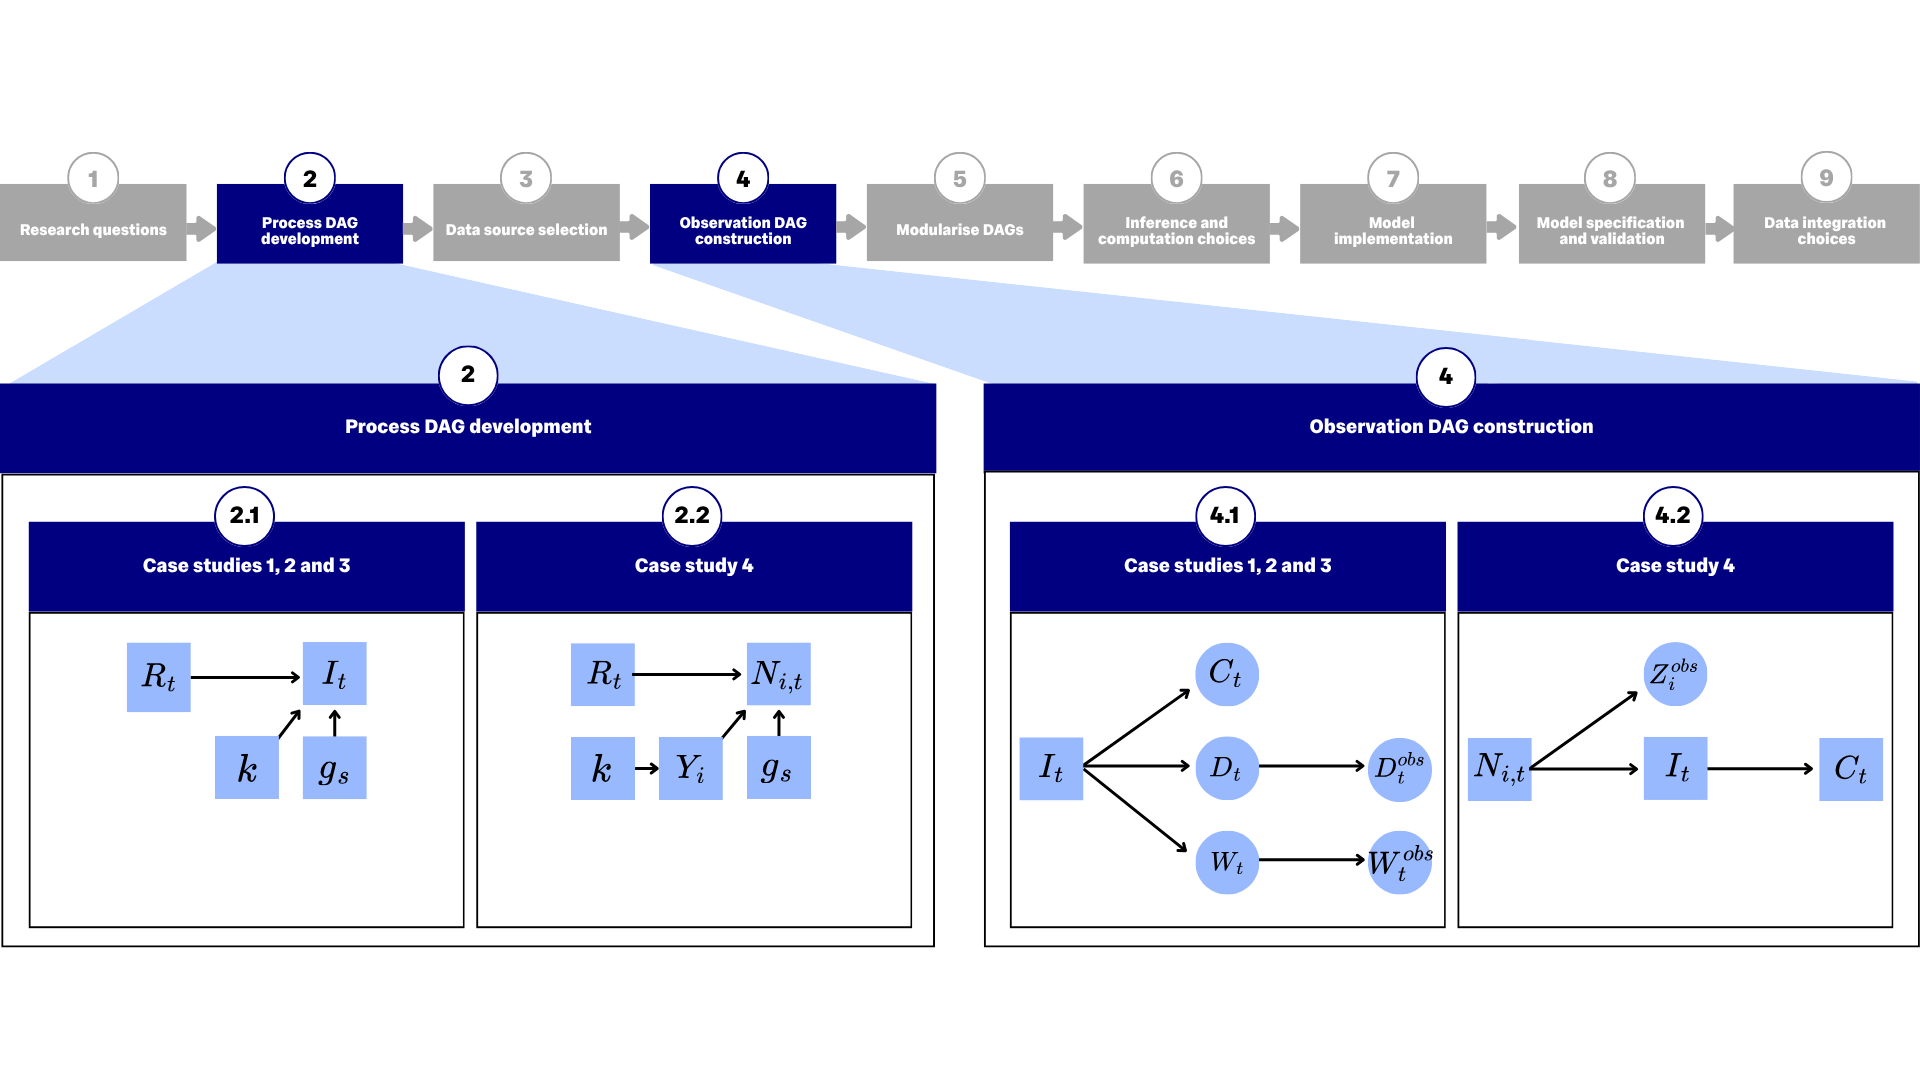
\includegraphics[width=\textwidth]{figures/Abbott et al figure 7.png}
    \caption{\textbf{A Schematic for Constructing the DAGs.} This schematic shows how data source selection and model choices can lead to different construction of the observation \ac{DAG} from the underlying process DAG for various case studies. For simplicity, feedback loops are omitted in this schematic. For a complete representation of feedback mechanisms, see Figure \ref{fig:workflow}.}
    \label{fig:case_study_diagram}
\end{figure}

\section{Discussion}
\label{sec:discuss}
%\subsection{Summary}

We have presented a suggested workflow for infectious disease modelling that addresses domain-specific challenges, extends established Bayesian workflow principles \citep{green2003highly,gelman2020bayesian}, and has a particular focus on integrating multiple data sources.
This workflow aims to serve as guidance for modellers when they are developing infectious disease models and as a resource for readers evaluating modelling papers, whether they work in academic research, public health agencies, or policy contexts that rely on model outputs.
We used four case studies to demonstrate this workflow using progressively more data sources for reproduction number estimation, showing how workflow practices can enable principled model development from single-source models to complex multi-stream integrations.
Each progression reinforces that additional data sources often alter both process and observation \ac{DAG}s and can require new integration, inference and implementation decisions.
Throughout, we highlight that considering each submodel in isolation is a useful starting point for model development and validation.

%\subsection{Strengths and Limitations/Outstanding Challenges}

The structure of our workflow addresses a critical gap in infectious disease modelling practice, where ad hoc approaches have often led to inadequate validation and limited transparency in methodological choices.
A key strength of our framework is the explicit separation of process and observation \ac{DAG}s in the spirit of state-space models, which provides clarity for model development and validation by recognising that epidemiological processes and observation mechanisms draw from different domains.
A significant limitation is that we have not implemented the workflow in practice, providing only schematic case studies that illustrate conceptual progression rather than actual code or examples.
Despite this lack of implementation, the framework's modular structure enables users to adopt specific components like our suggested data review process or DAG-based planning independently of other steps in their workflow.
In some sense, this lack of a specific tool example is a strength as it makes it easier to view this workflow as a guide, which can then be combined with tools of their choice.
Our structured data characterisation checklist provides an important benefit by establishing a common language for discussing data source trade-offs within modelling teams.
Yet this checklist is necessarily context-dependent, with criteria and their relative importance varying across pathogens, settings, and research questions.
This means that we cannot give an overview of all data sources, or even many common ones.
A limitation of our more specific implementation recommendations, such as which inference algorithm or \ac{PPL} to use, is that they will inevitably become outdated. However, the general principles underlying these recommendations, such as using gradient-based methods where applicable or implementing models in probabilistic programming frameworks, should remain useful, as should our broader recommendations for using a structured modelling workflow.
A final strength of our proposed framework is its applicability across diverse contexts, from early outbreak analysis to routine surveillance, offering a consistent structure regardless of data availability and research questions.


%\subsection{Comparison with Existing Literature}

Our workflow extends Gelman et al.'s general Bayesian workflow framework \citep{gelman2020bayesian}, which itself builds on wider statistical modelling workflows \citep{box1979robustness,Box1980,green2003highly}, by addressing workflow adoption challenges specific to infectious disease modelling.
Gelman et al. give a workflow for model validation and criticism within a single modelling cycle with extensive guidance and practical examples.
We embed their modelling loop within a larger workflow that aims to address domain-specific challenges: data source characterisation, integration strategies, and workflow iteration as outbreaks evolve. 
As noted, whilst we don't give fully implemented examples, we do provide additional domain-specific examples for surveillance data quality, reporting biases, and epidemiological process representation not covered in the general statistical literature.
 
Recent work has made progress towards structured infectious disease modelling workflows.
For example, \citet{bouman2024bayesian} systematically compared modelling choices for \ac{SARS-CoV-2} transmission and provided an open-source implementation.
However, they do not provide structured workflow guidance and key workflow elements such as prior predictive checks, systematic model criticism, and clear decision frameworks are absent.
Their work highlights the gap between implementing models and following robust and reproducible workflow practices.
In contrast, our framework provides explicit structured guidance through each workflow stage, with case studies demonstrating our decision process itself.
\citet{grinsztajn2021bayesian} provides systematic Bayesian workflow guidance for infectious disease transmission models in Stan, demonstrating prior predictive checks, inference criticism, and posterior predictive checks. 
Their workflow successfully integrates multiple data sources, including deaths, hospitalisations, and seroprevalence. 
However, their primary focus is on Stan implementation, and they mostly focus on implementing the Gelman et al. workflow without the infectious disease modelling modifications we have proposed.

Broader efforts have sought to standardise infectious disease modelling practice through consensus principles. \citet{Behrend2020-au} developed five key principles emphasising stakeholder engagement, reproducibility, data documentation, uncertainty communication, and testable model outcomes. 
Our workflow complements these principles by providing specific methodological guidance for technical decisions, particularly multi-source data integration.
Our structured approach, reporting recommendations and focus on modularity reflect their recommendations.

%\subsection{Future work}

Future progress requires infrastructure that makes it easier to implement methodological best practices.
Whilst this paper provides a schematic workflow, practical tutorials demonstrating actual implementation would make it easier to follow and likely identify weaknesses in our recommendations.
However, such tutorials and tools are likely to require advances in software composability, where self-contained components can be combined to build complex models, to make them feasible.
This would enable domain experts to contribute specialised components without rebuilding core functionality and make all steps of our proposed workflow easier to implement.
Improved tooling for Markov melding \citep{goudie2019joining} would facilitate modular integration, which would allow teams to more easily combine submodels without full joint specification or specialist knowledge. Further methodological work on cut posteriors \citep{liu2025general} is needed before easy-to-use tools to implement them can be developed.
Computational scalability remains an area where more work is needed, both for formal conflict detection \citep{yang2025detecting} and particularly for joint analysis of individual-level data with population surveillance.
Recent advances in inference algorithms, including gradient-free methods, adaptive sampling techniques, neural approaches for likelihood-free inference, and GPU-accelerated approaches, show promise for infectious disease modelling. However, more work is needed to evaluate existing advances and to develop new methods for scalable joint analysis of individual-level and population surveillance data, and methods that meet the real-time computational constraints of outbreak response.

%\section{Conclusions}

Our proposed workflow aims to address the slow adoption of rigorous practices that would benefit infectious disease modelling, by providing structured guidance for model development, validation, and multi-source integration that can adapt to evolving outbreak contexts.
The modular approach we advocate enables adding complexity incrementally whilst maintaining transparency about modelling assumptions and integration choices.
We recommend that the infectious disease modelling community adopt a structured workflow, such as the one presented here, for model development, evaluation, and reporting. 
This is particularly important during rapidly evolving outbreaks where research questions can change and new data sources emerge over time.

\section*{List of Abbreviations}
\begin{acronym}
  \acro{DAG}{Directed Acyclic Graph}
  \acro{MCMC}{Markov Chain Monte Carlo}
  \acro{HMC}{Hamiltonian Monte Carlo}
  \acro{NUTS}{No-U-Turn Sampler}
  \acro{VI}{Variational Inference}
  \acro{SMC}{Sequential Monte Carlo}
  \acro{SMC$^2$}{Sequential Monte Carlo Squared}
  \acro{POMP}{Partially Observed Markov Process}
  \acro{PMCMC}{Particle Markov Chain Monte Carlo}
  \acro{INLA}{Integrated Nested Laplace Approximation}
  \acro{MLE}{Maximum Likelihood Estimation}
  \acro{ABC}{Approximate Bayesian Computation}
  \acro{SL}{Synthetic Likelihood}
  \acro{BFMI}{Bayesian Fraction of Missing Information}
  \acro{ELBO}{Evidence lower bound}
  \acro{ESS}{Effective Sample Size}
  \acro{PPL}{Probabilistic programming language}
  \acro{LOO-CV}{leave-one-out cross-validation}
  \acro{WAIC}{Watanabe-Akaike information criterion}
  \acro{CRPS}{continuous ranked probability score}
  \acro{PMMH}{particle marginal Metropolis–Hasting}
 \acro{GPU}{Graphics Processing Unit}
 \acro{CPU}{Central Processing Unit}
 \acro{RNA}{Ribonucleic Acid}
 \acro{DNA}{Deoxyribonucleic Acid}
 \acro{PCR}{Polymerase Chain Reaction}
 \acro{ICU}{Intensive Care Unit}
 \acro{SARS-CoV-2}{Severe acute respiratory syndrome coronavirus 2}
\end{acronym}

\section{Acknowledgements}

We thank the organisers and participants of the workshop ``Analysis and modelling for the design of future epidemic surveillance systems'' (CIRM, Marseille, 28 April–2 May 2025) for valuable discussions and feedback that helped shape this work.
All workshop participants provided useful discussion and feedback.
We thank Poppy the dog for making sure to ask the important questions.
\pagebreak
\bibliographystyle{plainnat}
\bibliography{references,zotero-references}


\end{document}
 